\section{Analýza}
\subsection{Operačné systémy}
\indent Informatika a informačné technológie je pomerne mladá vedná disciplína. Jej začiatky je možné datovať od druhej polovice dvadsiateho storočia, čo momentálne predstavuje takmer sedemdesiat rokov. Za tento čas informatika zaznamenala enormný rast vo vývoji hardvéru, ako aj softvéru.  Operačný systém je základná časť akéhokoľvek počítačového sytému, predstavuje softvér, ktorý umožňuje počítačom pracovať. V poslednej dobe, oblasť operačných systémov  prechádza rapídnymi zmenami, pretože počítače sa stali súčasťou každodenného života, a to od malých zariadení, napríklad v automobiloch, až po najsofisitkovanejšie servery nadnárodných spoločností. Aj napriek tomu, že v dnešnej dobe poznáme mnohé operačné systémy, v práci sa zameriame na Windows, Mac OS, Unix a Linux.\cite{osbook}

\subsubsection{Windows}
\indent Microsoft Windows uviedol svoje prvé operačné systémy v novembri roku 1985 ako nadstavbu MS DOS. Jeho popularita rýchlo rástla až vyvrcholila dominantným postavením na trhu v osobných počítačoch. V roku 1993 začal vydávať špecializované operačné systémy, ktoré prinášali novú funkcionalitu pre počítače používané ako servery.\cite{windowsHistory} Pre účely automatizácie sa na Windows serveroch používajú hlavne powershell scripty, písané v rovnomennom jazyku Powershell\cite{winAutomation}.
\paragraph{Podiel na trhu}
\indent Microsoft je aj vzhľadom na svoju históriu najobľúbenejším operačným systémom v segmente osobných počítačov. Podľa webovej stránky statcounter.com\cite{statcounter} a netmarketshare.com\cite{netmarketshare} má 81,73\%  \acrshort{resp.}  88,42\% podiel na trhu.
\newline
\indent Podľa w3techs.com\cite{pop} je serverový operačný systém Windows používaný na 32.0\% počítačoch.
\paragraph{Predinštalovaný softvér}
\indent Windows operačné systémy ponúkajú základný balík nástrojov a programov. Serverové aj neserverové verzie Windowsu ponúkajú  Powershell, ktorý je dostupný od inštalácie.  Oba systémy podporujú aj takzvaný Command prompt alebo príkazový riadok, ktorý je alternatívou k Powershellu. Akékoľvek ďalšie programy je potrebné stiahnuť a doinštalovať.

\subsubsection{MacOs}
\indent  Mac okrem iného ponúka serverovú verziu operačného systému pod názvom OS X Server, ktorý začal písať svoju históriu v roku 2001, avšak neteší sa takej obľube ako Windows, Unix alebo Linux server. OS X server nepoužíva  špecifický skriptovací jazyk, pričom poskytuje možnosť výberu skriptovacieho jazyka, ako napríklad: Python, JavaScript, Perl, AppleScript, Swift alebo Ruby. Každý z uvedených jazykov prináša určité plusy, ako aj mínusy.
\paragraph{Predinštalovaný softvér}
\indent Predinštalovaný softvér pre developerov na Mac OS je Python, AppleScript, Ruby, Bash, BOjective-c. Donedávna bola štandardom aj Java, avšak Apple sa rozhodol pre radikálny krok vylúčiť Javu a propagovať Objective-c.
\paragraph{Podiel na trhu}
\indent Popularita počítačov s predinštalovaným operačným systémom MacOs sa mierne zvyšuje, čo je možné vidieť aj na obrázku na konci sekcie operačných systémov. Podľa webovej stránky statcounter.com\cite{statcounter} a netmarketshare.com\cite{netmarketshare} mu patrí 13,18\% resp.  9,19\% na trhu.
\indent Serverové verzie MacOs podľa stránky w3techs.com\cite{pop} sú na menej ako 0.1\% zariadeniach.
\subsubsection{Unix}
\indent Patrí medzi prvé operačné systémy pre servery, ktorého vývoj začal v roku 1970 a v priebehu rokov vzniklo veľa nových verzií Unixu a Linuxu. V minulosti boli Unixové servery veľmi obľúbené, avšak v súčasnosti sú na ústupe, a to najmä kvôli vyšším obstarávacím a prevádzkovým nákladom. Pre účely Unixu sa vytvoril Unix shell, dostupný v rôznych obmenách, ktorý je často vyhľadávaným jazykom medzi administrátormi a automatizačnými programátormi.
\paragraph{Predinštalovaný softvér}
\indent Na vačšine unixových systémoch je predinštalovaný Shell a Open JDK.
\paragraph{Podiel na trhu}
\indent Podľa stránky w3techs.com\cite{pop} sa Unixové systémy používajú na rovných 68.0\% počítačov.
\subsubsection{Linux}
\indent  Linux je všeobecný názov pre širokú zostavu Linux distribúcií, ktoré používajú Linux Kernel. Linux Kernel bol prvýkrát verejnosti predstavený v roku 1991 a odvtedy bol rozšírený na najviac platforiem. Momentálne je jediným používaným operačným systémom na TOP 500 superpočítačoch (mainframe). Skriptovacím jazykom pre Linux je Unix Shell resp. jeho najrozšírenejšia forma Bash.
\paragraph{Predinštalovaný softvér}
\indent Predinštalovaný softvér vo väčšine distribúciách Linuxu sú Bash, Open JDK - Java, niektoré distribúcie ponúkajú Python. RedHat začína s podporou .NET frameworku.
\paragraph{Podiel na trhu}
\indent Linux je k dispozícii v mnohých formách, tak aby vyhovoval rôznym potrebám, od spotrebiteľsky orientovaných systémov pre domáce použitie až po distribúcie použiteľné v špecifických odvetviach. Podľa webovej stránky statcounter.com\cite{statcounter} a netmarketshare.com\cite{netmarketshare} mu patrí 1,66\% resp.  1,93\%.
Podľa stránky w3techs.com\cite{pop} je operačný systém Linux na 41.0\% počítačoch.
\subsubsection{Porovnanie podielov operačných systémov}
\indent Nasledujúce grafy zobrazujú podiel operačných systémov na trhu v segmente osobných počítačov, ako aj v segmente serverov. Zaujímavý graf je vývoj trendu využívania serverových operačných systémov, z ktorého vidíme, že unixové a linuxové servery zvyšujú svoje podiely na trhu. Naopak, Windows v posledných mesiacoch stratil pár percent. Taktiež je vidieť, že linuxové a unixové systémy pokrývajú viac ako polovicu web stránok, ktoré majú najvyššie hodnotenie. Je potrebné dodať, že percentá na posledných dvoch obrázkoch pre Unix a Linux, nemožeme sčítavať, nakoľko na w3techs berú Linux ako podmnožinu Unix \acrshort{os}. Teda napríklad štatistika z predposledného obrázku hovorí, že podiel Unixu na trhu je 68\% z toho väčšiu časť tvorí práve \acrshort{os} Linux s 41.1\% podielom.
\begin{figure}[!htbp]
	\centering
	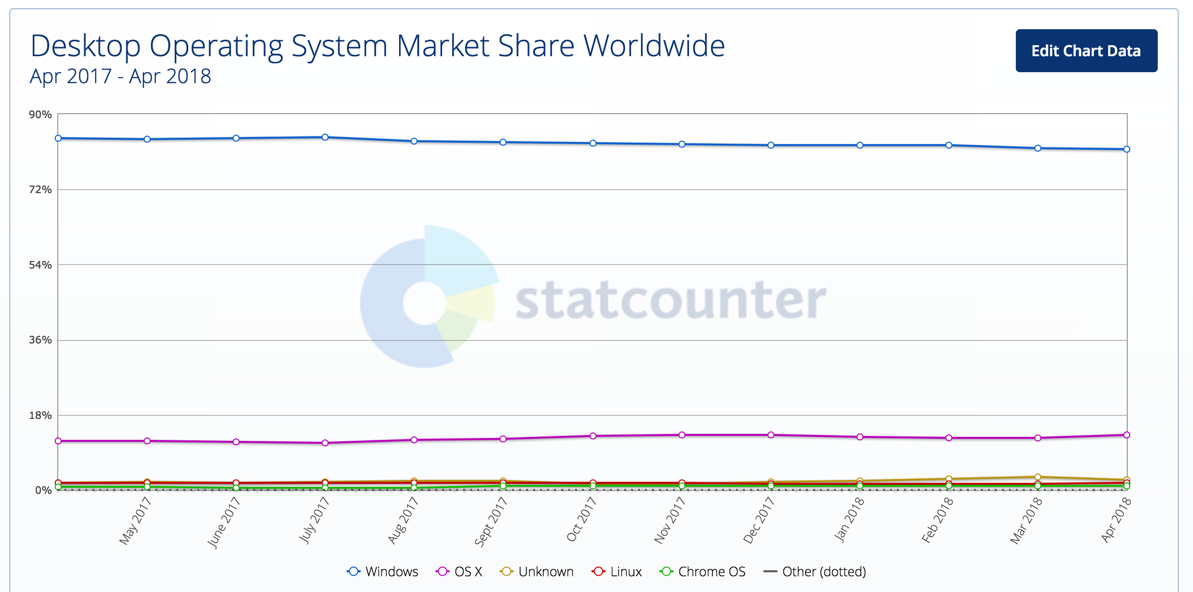
\includegraphics[width=\linewidth]{img/statcounter.png}
	\caption{\acrshort{os} - podiel na trhu podľa statcounter\cite{statcounter}}
	\label{fig:test}
	
\end{figure}
\begin{figure}[!htbp]
	\centering
	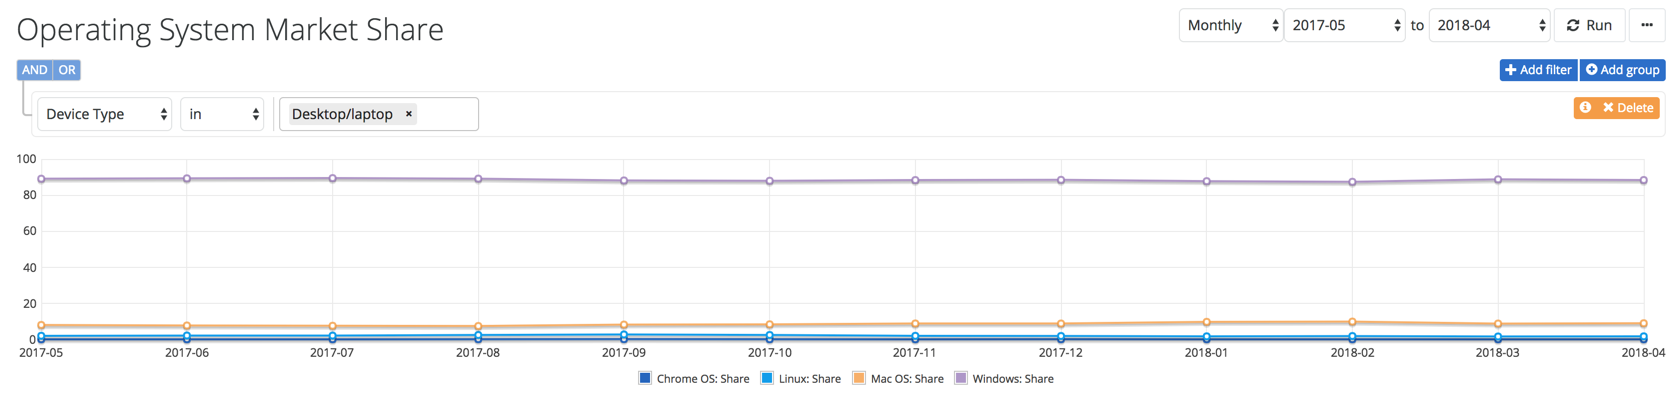
\includegraphics[width=\linewidth]{img/netmarketshare.png}
	\caption{\acrshort{os} - podiel na trhu podľa netmarketshare\cite{netmarketshare}}
	\label{fig:test}
	
\end{figure}
\begin{figure}[!htbp]
	\centering
	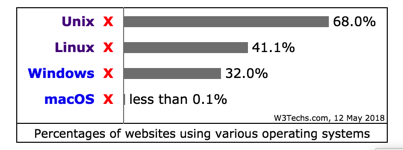
\includegraphics[scale=0.4]{img/usg_server.png}
	\caption{Serverové \acrshort{os} - podiel na trhu podľa w3techs\cite{pop}}
	\label{fig:test}
	
\end{figure}
\begin{figure}[!htbp]
	\centering
	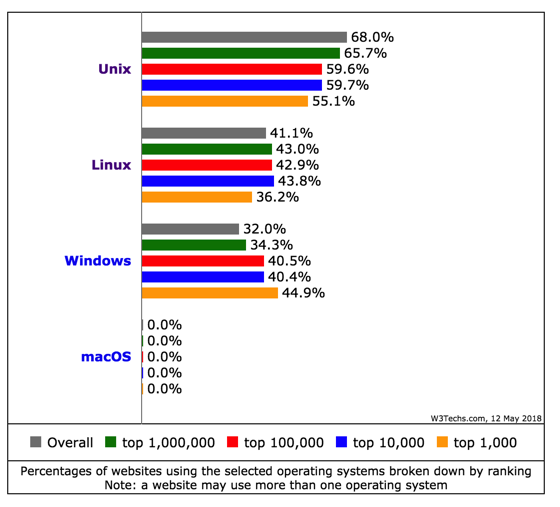
\includegraphics[scale=0.4]{img/usage_grou_by_os_sites.png}
	\caption{Serverové \acrshort{os} - podiel na trhu a rozdelenie podľa hodnotenia stránok podľa w3techs\cite{pop}}
	\label{fig:test}
	
\end{figure}

\subsection{Programovacie jazyky}
\indent S príchodom osobných počítačov, no najmä serverov, sa programátori zaujímali o automatizáciu procesov, ktoré na danom stroji bolo spočiatku potrebné spúšťať manuálne. Keďže tieto úlohy neboli natoľko komplexné ako samotné programy, ktoré spúštali, bolo vhodné na úlohy využiť a vytvoriť skriptovacie jazyky. V nasledujúcej časti priblížime niekoľko programovacích jazykov, ktoré sa v dnešnej dobe bežne používajú na tvorbu automatizovaných skriptov.

\subsubsection{Shell}
\indent
Je skriptovací jazyk pre unixové distribúcie, ktorý do súčasnosti prešiel rôznymi zmenami a rozšíreniami. Verzie Shellu predstavujú: sh, csh, ksh,tcsh, bash. Verzia Bash je momentálne najobľúbenejšou, avšak zsh je verzia Shellu, ktorá má najviac rôznych rozšírení funkcionality, ako aj veľa priaznivcov medzi developermi. V nasledujúcich častiach všeobecne zhodnotíme jednotlivé výhody a nevýhody skriptovacieho jazyka Shell.

\paragraph{Výhody}
\begin{itemize}
	\item automatizácia často opakujúcich sa úloh,
	\item možnosť zbiehať zložené príkazy, ako jednoriadkový príkaz  - tzv. reťazenie príkazov,
	\item jednoduchý jazyk na používanie,
	\item výborne spracované manuálové stránky,
	\item Unix Shell je portabilný naprieč platformami Linuxu/Unixu,
	\item jednoduché plánovanie automatických úloh.
	\newline
\end{itemize}
\paragraph{Nevýhody}
\begin{itemize}
	\item najväčšou nevýhodou je skutočnosť, že prirodzene nefunguje pod Windows OS, pričom na sprostredkovanie funkcionality používa rôzne emulátory a nástroje tretích strán,
	\item pomalé vykonávanie príkazov pri porovnaní s inými programovacími jazykmi,
	\item nový proces pre skoro každý spustený príkaz,
	\item zložitejší na zapamätanie rôznych prepínačov, ktoré dané príkazy podporujú,
	\item nejednotnosť prepínačov,
	\item neprenosný medzi platformami,
	\item Shell nepridáva vlastné príkazy, používa len tie, ktoré sú dostupné na konkrétnom počítači.
\end{itemize}
\paragraph{Popis a zhodnotenie jazyka}
\indent
Unix Shell je obľúbeným scriptovacím jazykom, vhodným na automatizovanie každodenných operácií. Je jedným z najpoužívanejších skriptovacích jazykov, nakoľko všetky Linuxové, Unixové servery využívajú práve tento jazyk ako svoj primárny. V nasledujúcich častiach popíšeme Bash, ktorý je najrozšírenejšou verziou Unix Shell. Zaujímavou prednosťou jazyka je pajpa. Pajpa je klasický príklad vnútro-procesorovej komunikácie: odovzdáva štandardný výstup stdout procesu na štandardný vstup stdin iného procesu, viď príklad.
\begin{minted}[]{php}
zarrelli:~\$ ls -lah | wc -l
35
\end{minted}
V uvedenom príklade sme vylistovali obsah adresára, v ktorom sa práve nachádzame, a výstupom z programu sme naplnili štandardný vstup aplikácie "wc", ktorá spočíta, koľko riadkov sa nachádza na vstupe, ktorý jej bol dodaný. Príkaz za znakom pajpy | zbieha v Subshell-i, čo znamená, že nebude schopný zmodifikovať hodnoty v rodičovskom procese. Zlyhanie príkazu v pajpe vedie k takzvanej "zlomenej pajpe", v tomto prípade exekúcia príkazov skončí. \cite{mbash}
\newpage
Taktiež niektoré často používané príkazy majú zmenený spôsob zápisu.
Ako príklad si uvedieme príkaz for, pri ktorom bash používa následovnú Syntax:

\begin{algorithm}[H]
	\begin{minted}{php}
	#!/bin/bash
	// prvý spôsob zápisu podobná vylepšenej verzii z predchádzajúceho príkladu
	for placeholder in list_of_items
	do
	action_1 \$placeholder
	action_2 \$placeholder
	action_n \$placeholder
	done
	//kolekcia vo fore môze byť reprezentovaná vymenovaním prvkov 
	//priamo za "in" časťou
	for i in 1 2 3 4 5
	do
	echo "\$i"
	done
	// c-like prístup
	for ((i=20;i > 0;i--))
	{
	if (( i % 2 == 0 ))
	then
	echo "\$i is divisible by 2"fi
	}
	exit 0
	\end{minted} 
	\caption{Bash ukážka rôznych volaní for cyklu. \cite{mbash}}
	\label{alg:gen}
\end{algorithm}

Ako vidíme z príkladu, for používa podobnú Syntax ako ostatné jazyky, a ďalej ju rozširuje. Vyššie spomenuté použitia niesú jediné, kde druhý spôsob môže uľahčiť prácu napríklad pri prototypovaní skriptu, v ktorom Shell poskytuje možnosť vložiť parametre pre cyklus priamo z konzoly ako v nasledujúcom príklade.
\newpage
\begin{algorithm}[H]
	\begin{minted}{php}
	//telo skriptu
	#!/bin/bash
	i=0
	for cities 
	do
	echo "City $((i++)) is: $cities"
	done
	exit 0
	
	//následné volanie z konzoly
	./for-pair-input.sh 
	Belfast Redwood Milan Paris
	City 0 is: Belfast
	City 1 is: Redwood
	City 2 is: Milan
	City 3 is: Paris
	\end{minted}
	\caption{Bash ukážka volania skriptu s for cylom priamo z konzoly . \cite{mbash}}
	\label{alg:gen}
\end{algorithm}

Syntax jazyka je náročnejšia na učenie, pretože používa rôzne prepínače, ktoré novému používateľovi nemusia byť sprvu jasné. 
V tabuľke uvádzame príklad prepínačov pre if, ktorý pre podmienkovú časť používa hranaté zátvorky namiesto okrúhlych, na ktoré sme zvyknutí z väčšiny programovacích jazykov. Je potrebné spomenúť, že napríklad Unix shell nepoužíva žiadne zátvorky v podmienkovej časti príkazu, na ukončenie podmienkovej časti sa používa bodkočiarka, čo spôsobuje problémy pri prenositeľnosti. If ponúka aj ďalšie prepínače, no zhodnotili sme, že pre ilustráciu budú postačovať aj príklady uvedené v tabuľke.
Najvačsia nevýhoda je, že Shell script nie je multiplatformový jazyk, a teda ak by sme mali prostredie, v ktorom servery bežia na rôznych operačných systémoch, potrebovali by sme poznať ďalší jazyk, ktorým by sme docielili rovnaké alebo aspoň podobné výsledky.
\newline
\begin{table}[h!]
	\centering
	\begin{tabular}{|p{4cm}|p{13cm}|}
		\hline
		Reťazcové porovnanie & Popis \\
		\hline
		Str1 = Str2	& Vráti true, ak sa porovnávané reťazce rovnajú. \\ 
		\hline
		Str1 != Str2 &	Vráti true, ak porovnávané reťazce nie sú rovnaké.\\ 
		\hline
		-n Str1	 &R Vráti true, ak reťazec nie je null resp. o dĺžke 0.\\ 
		\hline
		-z Str1	& Returns true, ak reťazec je null resp. o dĺžke 0.\\
		\hline
	\end{tabular}
	\caption{Ukážka reťazcových prepínačov v podmienkovom výraze if \cite{shellprep}}
	\label{table:1}
	
\end{table}
\begin{table}[h!]
	\centering
	\begin{tabular}{|p{4cm}|p{13cm}|}
		\hline
		Numerické porovnanie	& Popis \\
		\hline
		expr1 -eq expr2	& Vráti true, ak sú porovnávané výrazy rovné. \\
		\hline
		expr1 -ne expr2	& Vráti true, if ak nie sú porovnávané výrazy rovné. \\
		\hline
		expr1 -gt expr2	& Vráti true, ak je hodnota premmenej expr1 väčšia než hodnota premennej expr2. \\
		\hline
		expr1 -ge expr2	& Vráti true, ak je hodnota premmenej expr1 väčšia alebo rovná hodnote premennej expr2. \\
		\hline
		expr1 -lt expr2	& Vráti true, ak je hodnota premmenej expr1 menšia než hodnota premennej  expr2. \\
		\hline
		expr1 -le expr2	& Vráti true, ak je hodnota premmenej expr1 menšia alebo rovná hodnote premennej expr2. \\
		\hline
		! expr1	& Operátor "!" zneguje hodnotu premennej expr1. \\
		\hline
	\end{tabular}
	\caption{Ukážka numerických prepínačov v podmienkovom výraze if \cite{shellprep}}
	\label{table:1}
	
\end{table}
\newpage

\subsubsection{Powershel/Classic command line}
\indent  
Command line je základným skriptovacím jazykom pre Windows distribúcie, ktorý poskytuje malé \acrshort{api} pre svojich používateľov. Aj kvôli uvedenej skutočnosti Miscrosoft predstavil nový jazyk Powershell. Powershell je kombináciou príkazového riadku, funkcionálneho programovania a objektovo-orientovaného programovania. Je založený na .NET frameworku, ktorý mu zabezpečuje istú mieru flexibility. 
Výhody a nevýhody Powershell zhrnieme v nasledujúcich častiach.

\paragraph{Výhody}
\begin{itemize}
	\item bohaté \acrshort{api},
	\item výborne riešený run-time,
	\item flexibilita,
	\item veľmi jednoduché prepnúť z .NET frameworku,
	\item dokáže pridávať funkcionalitu používaním tried a funkcií z .NET knižníc.
	\newline 
\end{itemize}
\paragraph{Nevýhody}
\begin{itemize}
	\item bohaté \acrshort{api} - nejednoznačné, kedy čo použiť,
	\item niektoré výhody jazyka sú až nevhodne skryté pred používateľmi,
	\item staršie verzie serverov nie sú Powershell-om podporované tak, ako novšie,
	\item horšia dokumentácia v porovnaní so Shell scriptom.
	\newline
\end{itemize}

\paragraph{Popis a zhodnotenie jazyka}
Powershell je obľúbený medzi programátormi a administrátormi, ktorí pracujú pod operačným systémom Windows. Donedávna, kým Powershell fungoval na .NET frameworku, ho nebolo možné používať mimo operačných systémov Windows. Avšak s príchodom frameworku .NET Core sa situácia zmenila. Spomenutý frawework je momentálne open source, jeho zdrojové kódy boli zverejnené a je možné do neho prispievať. Okrem iného, podporuje rovnaké alebo aspoň podobné štruktúry ako Shell script. V niektorých prípadoch poskytuje rovnaké príkazy, napríklad: mv, cp, rm, ls. Jedným zo zásadných rozdielov medzi Shellom a Powershellom je skutočnosť, že kým v Shelli sú pre vstup aj výstup používané textové reťazce, ktoré je potrebné rozparsovať a interpretovať, v Powershelli je všetko presúvané ako objekt. Ide o najzásadnejší rozdiel, nakoľko ostatné veci boli pravdepodobne navrhované v spolupráci s používateľmi Shell scriptu. \cite{psbook}

Pre demonštráciu rozdielov pri odovzdávaní parametrov medzi príkazmi uvádzame príklad.
\newpage
\begin{algorithm}[H]
	\begin{minted}[]{php}
	function changeName(\$myObject)
	{
	if (\$myObject.GetType() -eq [MyType])
	{
	//vypíš obsah premennej
	\$myObject.Name
	//zmeň reťazec pre atribút name
	\$myObject.Name = "NewName"
	}
	return \$myObject
	}
	
	// Vytvorenie objektu s argumentom OriginalName a následné použitie funkcie na zmenu argumentu
	//PS> \$myObject = New-Object MyType -arg "OriginalName"
	//PS> \$myObject = changeName \$myNewObject
	//OriginalName
	//PS> \$myObject.Name
	//NewName
	// Ukážka s využitím pipe
	//PS> \$myObject = New-Object MyType -arg "OriginalName" | changeName
	//OriginalName
	//PS> \$myObject.Name
	//NewName
	\end{minted}
	\caption{Ukážka použitia pipe v Powershell. \cite{netalg}}
	\label{alg:gen}
\end{algorithm}

\subsubsection{Python}
\indent Do analýzy sme zahrnuli aj programovací jazyk Python. Výber Python-u nebol náhodný, kedže je jedným z najpopulárnejších programovacích jazykov súčasnosti. Je viacúčelový, patrí mezi vyššie programovacie jazyky, objektovo-orientovaný, interaktívny, interpretovaný a extrémne používateľsky prijateľný.\cite{python}
\paragraph{Výhody}
\begin{itemize}
	\item je ľahko čitateľný, tým pádom ľahšie pochopiteľný,
	\item Syntax orientovaná na produktivitu,
	\item multiplatformový - po inštalácii interpretera,
	\item obsahuje množstvo rôznych knižníc,
	\item Open source.
	\newline
\end{itemize}
\paragraph{Nevýhody}
\begin{itemize}
	\item rýchlosť,
	\item slabšia dokumentácia,
	\item nevhodný pre úlohy pracujúce s vyšším množstvom pamäte,
	\item nevhodný pre viac-procesorovú prácu,
	\item nevhodný pre vývoj na mobilných zariadeniach,
	\item limitovaný prístup k databázam.
	\newline
\end{itemize}

\paragraph{Popis a zhodnotenie jazyka}
\indent Ako už bolo spomenuté, Python je jedným z najobľúbenejších jazykov súčasnosti, kde prevažnú časť komunity tvoria vedci, ktorí nemajú rozsiahle programátorské znalosti. Práve jednoduchosť, čitateľnosť a pochopiteľnosť jazyka sa značnou mierou podieľajú na tomto fakte. Rovnako Python nevyžaduje manažovať pamäť a iné netriviálne záležitosti nižších programovacích jazykov. Aj napriek tomu, že jazyk je objektovo-orientovaný, skripty sa v ňom píšu jednoducho. Poskytuje štruktúry ako pajpa, možnosť pracovať s procesmi, vytvárať triedy, inštancie, jednoducho prototypovať a simulovať rôzne problémy. Veľkou výhodou tohto jazyka je, že je open source s veľkou komunitou, ktorá rada testuje nové vydania, nahlasuje problémy, tým pádom je jazyk rýchlejšie a kvalitnejšie vyvíjaný. Na Python-e vznikli zaujímavé webové frameworky, ako napríklad Django. Každá strana má dve mince, a ani Python nie je stopercentný. Tým, že predstavuje interpretovaný jazyk, neprekypuje rýchlosťou. Veľa ľudí sa zaoberá rýchlosťou jazykov, zisťujú efektívnosť pri rôznych úkonoch, ako napríklad cykly, volania funkcií, aritmetika, prístup k pamäti, vytváranie objektov. V nasledujúcich tabuľkách je možné porovnať rozdiel v rýchlosti jednotlivých testov. 
\begin{center}
	\begin{table}[htbp]
		\begin{tabular}{|p{3.5cm}|p{3.5cm}|p{3.5cm}|p{3.5cm}|}
			\hline
			\textbf{Jazyk} & \textbf{Force field benchmark}  & \textbf{Array reverse benchmark}&\textbf{Rolling average benchmark} \\ 
			\hline
			C++ (-O2)&1.892&4.367&0.005\\
			\hline
			Java 7&2.469&3.776&0.463\\
			\hline
			C\# (normal)&10.712&14.071&0.621\\
			\hline
			JavaScript&16.159&13.162&1.312\\
			\hline
			Python 2&717.2&1485&71.550\\
			\hline
			Python 3&880.7&1466&81.143\\
			\hline
		\end{tabular}
		\caption{Porovnanie rýchlostí rôznych jazykov\cite{gitspeed}}
		\label{table:1}
	\end{table}
\end{center}
Aj keď sme spomenuli viaceré nedostatky, asi najväčším je rýchlosť. Ďalším nedostatkom je kolísanie syntaxe medzi jednotlivými verziami jazyka, čo má za následok nevyhnutnosť úpravy už preddefinovaných skriptov. Aj keď Python podporuje verzovanie knižníc, na \acrshort{pc} je možné mať iba jednu verziu. Výhodnejšie je mať všetky verzie danej knižnice a v hlavičke skriptov definovať verziu, ktorú je potrebné pre daný skript použiť. V takomto prípade by bola zabezpečená spätná kompatibilita, ktorú ale Python nemá.
\subsection{Existujúce riešenia}
\indent
Existuje množstvo emulátorov a nástrojov tretích strán, ktoré sprostredkúvajú funkcionality Shell scriptu do Windowsu, niektoré z nich si predstavíme.

\subsubsection{ConEmu}
\indent ConEmu je konzolový emulátor, ktorý poskytuje jednoduché \acrshort{gui}, do ktorého je možné vložiť viacero konzol. Dokáže spúšťať jednoduché \acrshort{gui} aplikácie, ako napríklad Putty, Cygwin. Obsahuje množstvo nastavení, ako nastavenie kurzora, priehľadnosti, písma a pod. Podporuje Windows 2000 a neskoršie verzie. Neposkytuje verziu pre iné operačné systémy. \cite{conemu}
\paragraph{Skúsenosti}
\indent ConEmu je vydarený emulátor, ktorý je schopný vykonávať akýkoľvek skript. Používaním sme neprišli na závažné nedostatky, ktoré by neboli popísané v issues logu na Githube. Tak ako každý softvér, aj ConEmu je náchylný na chyby. Podľa issues logu sa do oficiálnych vydaní dostávajú rôzne problémy, ktoré neboli zahrnuté v predchadzajúcich verziách. V tomto prípade je na zvážení každého používateľa, či aj napriek problémom, ktoré sa môžu dostávať do jednotlivých verzií emulátora, použije ConEmu, resp. či jeho kladné stránky prekonajú tie záporné.

\begin{figure}[!htbp]
	\centering
	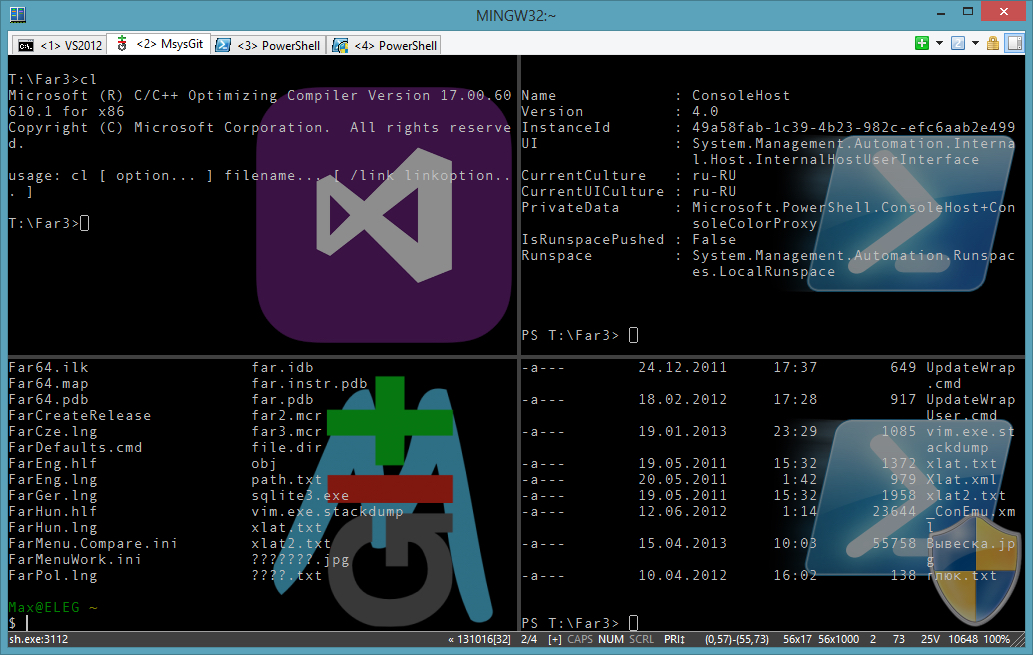
\includegraphics[scale=0.3]{img/conEmuImg.jpg}
	\caption{Ukážka ConEmu emulátora}
	\label{fig:test}
\end{figure}
\newpage
\subsubsection{cmder}
\indent Cmder je ďalším príkladom emulátora Shell terminálu. Vychádza z troch projektov ConEmu, Clink a Git pre Windows - voliteľná súčasť. ConEmu sme si predstavili v predcházajúcej časti spolu s jeho kladmi a zápormi. Clink, konkrétne Clink-completions je v projekte využívaný na zvýšenie komfortu pri písaní skriptov, nepridáva ďalšiu Shell funkcionalitu. \cite{cmder}
\paragraph{Skúsenosti}
\indent ConEmu je príjemný nástroj, dokáže zjednodušiť prácu, obzvlášť ak je používateľ zvyknutý na programovanie v Shell scripte. Keďže Cmder používa ConEmu ako emulátor Shell terminálu, a je určený pre Windows platformu, nemožno hovoriť o multiplatformovom riešení.
\begin{figure}[!htbp]
	\centering
	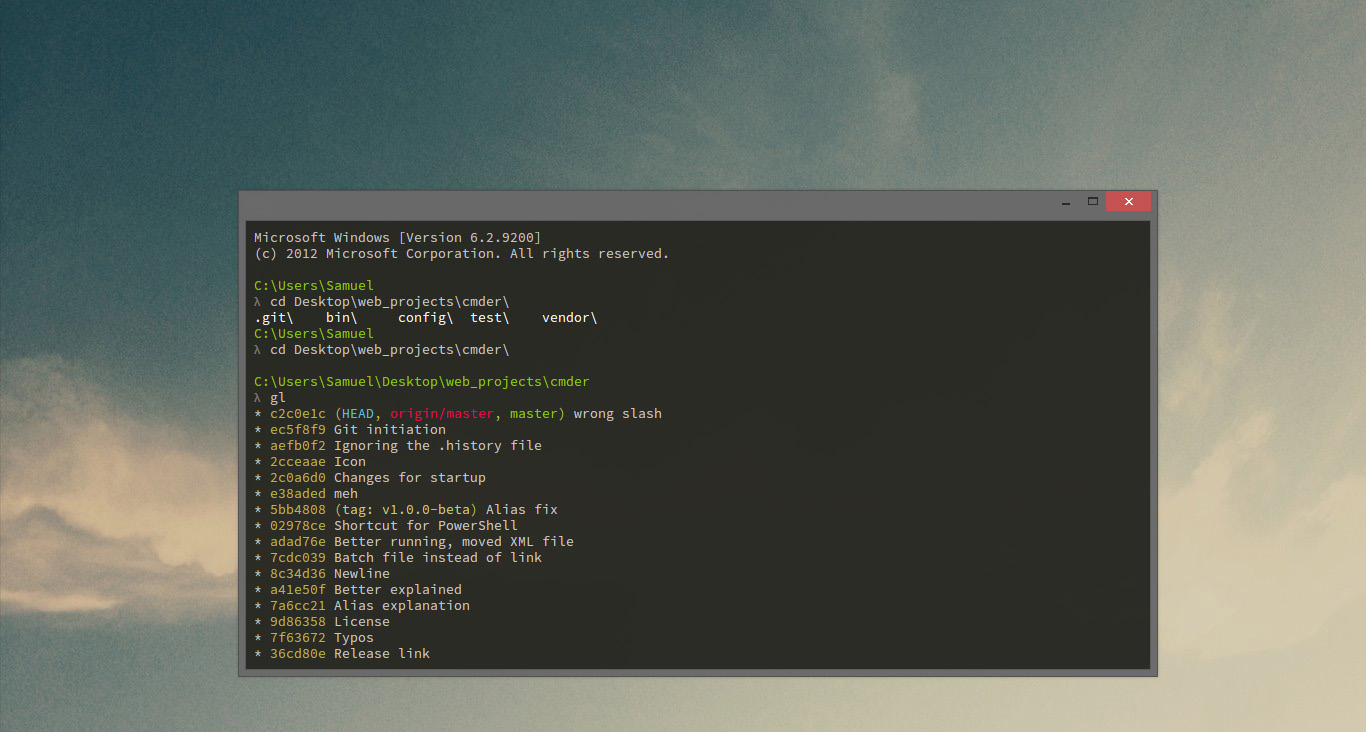
\includegraphics[scale=0.3]{img/cmder.jpg}
	\caption{Ukážka Cmder emulátora}
	\label{fig:test}
\end{figure}
\newpage
\subsubsection{Babun}
\indent Babun je jedným z mnohých emulátorov pre Windows, ktorý je nadstavbou cygwinu. Vo svojom jadre používa zshell a bash, ktoré sme popísali ako populárne medzi komunitou. Prináša vlastné \acrshort{gui}, ktoré dokáže zafarbovať text podľa zdrojového jazyka, čo zvyšuje prehľadnosť. Obsahuje git, svn, python, perl. Tiež má integrované sťahovanie nových balíčkov, ktoré ponúka cygwin pomocou kľúčového slova pact. Prenositeľnosť skriptov z unixových strojov je zabezpečená tým, že používa bash a zsh, avšak je to emulátor výhradne pre Windows distribúcie.\cite{babun}
\begin{figure}[!htbp]
	\centering
	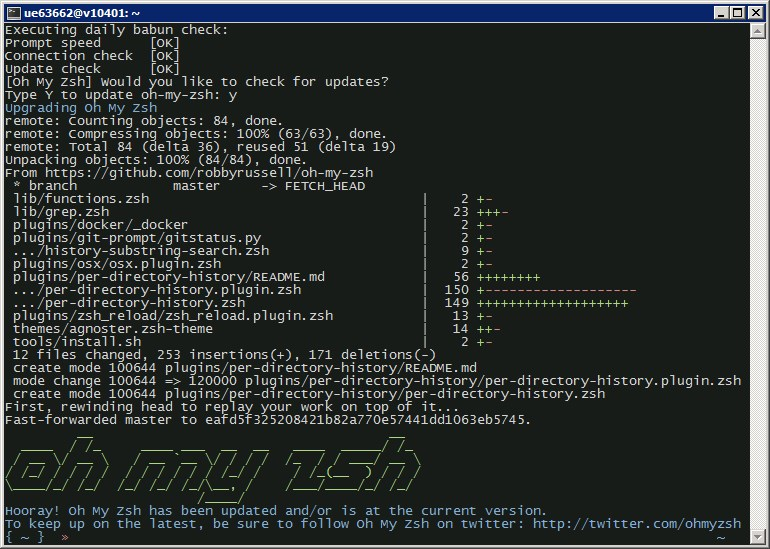
\includegraphics[scale=0.4]{img/babun.jpeg}
	\caption{Ukážka Babun emulátora}
	\label{fig:test}
\end{figure}
\subsubsection{MobaXterm}
\indent Poskytuje množstvo funkcionalít, avšak je zaťažený licenciou v hodnote 50 eur. \cite{mobaxterm}
\paragraph{Neplatená verzia}
\begin{itemize}
	\item Plná podpora SSH a X serveru
	\item Vzdialená plocha (RDP, VNC, Xdmcp)
	\item Vzdialený terminál (SSH, telnet, rlogin, Mosh)
	\item X11-Forwarding
	\item Automatický SFTP prehliadač
	\item Podpora pluginov
	\item Možnosť inštalovateľnej alebo prenositeľnej verzie
	\item Plná dokumentácia
	\item Maximálne 12 spojení
	\item Maximálne 2 SSH tunely
	\item Maximálne 4 makrá
	\item Maximálne 360 sekúnd pre Tftp, Nfs a Cron
\end{itemize}

\paragraph{Platená verzia}

\begin{itemize}
	\item Všetky vymoženosti z neplatenej verzie Home Edition +
	\item Možnosť upraviť uvítaciu správu a logo
	\item Modifikovať profilový skript
	\item Odstrániť nechcené hry, šetriče obrazovky alebo nástroje
	\item Nelimitovaný počet spojení
	\item Nelimitovaný počet tunelov a makier
	\item Nelimitovaný čas behu pre sieťové daemony
	\item Podpora centrálneho hesla
	\item Profesionálna technická podpora
	\item Doživotné právo používania
\end{itemize}

\subsection{Zhodnotenie analyzovaných technológií}
\indent Analýza ukázala, že väčšinový podiel na trhu osobných počítačov, ako aj serverov, tvoria Unix/Linux a Windows operačné systémy. Preto boli objektom analýzy hlavne programovacie jazyky, ktoré sú obľúbené medzi administrátormi daných jazykov. Ďalej sme preskúmali rôzne dostupné riešenia problému univerzálnej konzoly, z čoho usudzujeme, že ani jeden z produktov neposkytoval kompatibilitu na oboch alebo viacerých systémoch, maximálne kopíroval funkcie jedného systému do druhého. Na základe týchto poznatkov, ako aj poznatkov podrobnejšie rozpísaných v predchádzajúcich častiach, sme sa rozhodli pokračovať v analýze prekladu jazykov a získané vedomosti zúročiť do vlastného univerzálneho, platformovo nezávislého konzolového rozhrania.


\section{Preklad jazykov}
\indent Pri programovacích jazykoch nás zaujímajú ich vyjadrovacie schopnosti ako aj vlastnosti z hľadiska ich rozpoznania. Tieto vlasnosti sa týkajú programovania a prekladu, pričom obe je potrebné zohľadniť pri tvorbe jazyka. V dnešnej dobe sa používajú na programovanie hlavne takzvané vyššie programovacie jazyky, môžeme ich označiť ako zdrojové jazyky. Na to aby vykonávali čo používateľ naprogramoval je potrebné aby boli pretransformované do jazyka daného stroja. Spomínanú transformáciu zabezpečuje prekladač, prekladačom máme na mysli program, ktorý číta zdrojový jazyk a transformuje ho do cieľového jazyka, ktorému rozumie stroj.\cite{gram}

\subsection{Kompilátor proces prekladu}
Aby bol preklad možný, musí byť zdrojový kód programu napísaný podľa určitých pravidiel, ktoré vyplývajú z jazyka. Proces prekladu je možné rodeliť na 4 hlavné časti.
\begin{itemize}
	\item lexikálna analýza
	\item syntakticka analýza
	\item spracovanie sémantiky
	\item generovanie cieľového jazyka
\end{itemize}
\indent Podrobnejšie si stručne popíšeme všetky štyri časti, ktoré majú pre nás z hľadiska prekladu najväčší zmysel.
\newline
\subsubsection{Lexikálna analýza}
	\indent Lexikálna analýza je prvou fázou kompilátora. Dopredu napísaný zdojový kód je postupne spracovávaný preprocesorom, ktorý vytvára takzvané lexémy. 
	 \newline Lexémou nazývame postupnosť alfanumerických znakov. Tieto postupnosti znakov sú následne vkladané do lexikálneho analyzátora, ktorý ma za úlohu vytvoriť zo vstupných lexém tokeny slúžiace ako vstup pre syntaktický analyzátor. 
	 \newline Tokeny sa vytvárajú na základe preddefinovaných pravidiel, ktoré sa v programovacích jazykoch definujú ako pattern. V prípade, že lexikálny analyátor nieje schopný nájsť  pattern pred danú lexému musí vyhlásiť chybu počas tokenizácie.  
	 \newline Výstupom z lexikálnej analýzy sú takzvané tokeny, ktoré tvoria vyššie jednotky jazyka ako kľúčové slová jazyka, konštanty, identifikátory, operátory a iné.\cite{gram}
	 
	 \begin{figure}[!htbp]
	 	\centering
	 	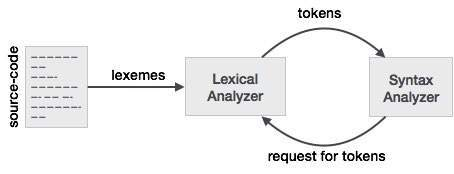
\includegraphics[width=15cm]{img/lexical_analysis.jpg}
	 	\caption{Ukážka práce lexikálneho analyzátora}
	 	\label{fig:test}
	 \end{figure}
 \newline
 
\subsubsection{Syntaktická analýza}
\indent Ďalšou fázou je syntaktická analýza. Úlohou Syntaktického analyzátora je kontrola správnosti vytvorených tokenov s uchovaním niektorých získaných informácií o štruktúre skúmanej syntaktickej jednotky. Syntaktická analýza sa radí medzi bezkontextové gramatiky. Po skoncení syntaktickej analýzy prichádza na rad sémantická analýza.\cite{gram}

 \newline
  \newline
\begin{figure}[!htbp]
	\centering
	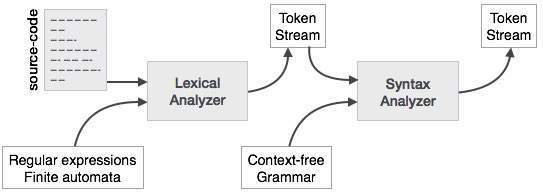
\includegraphics[width=15cm]{img/syntax_analyzer.jpg}
	\caption{Ukážka práce syntaktickeho  analyzátora}
	\label{fig:test}
\end{figure}
 \newline
 \newpage
\subsubsection{Limitácia syntaktickej analýzy}
\indent Syntaktický analyzátor ziska vstup z tokenu, ktorý vytvorí lexikálny analyzátor. Lexikálne analyzátory sú zodpovedné za validitu tokenu.Syntaktické analyzátory majú nasledovné limitácie.

\begin{itemize}
	\item nedokážu zistiť validitu tokenu
	\item nedokážu zistiť či je token používaný pred tým ako je deklarovaný
	\item nedokážu zistiť či je token používaný pred tým ako je inicializovaný
	\item nedokážu zistiť validitu operácie, ktorú token vykonáva
\end{itemize}



\subsubsection{Semantická  analýza}
\indent Sémantická analýza má za úlohu interpretovať symboly, typy, ich vzťahy.Sémantická analýza rohoduje či má syntax programy význam alebo nie.
Ako príklad zisťovania významu môžeme uviesť jednoduchú inicializáciu premennej.\cite{gram}

\begin{lstlisting}

	int integerVariable = 6

	int secondIntegerVariable = "six"
\end{lstlisting}

Oba príklady by mali prejsť cez lexikálnu a syntaktickú analýzu. Je až na sémantickej analýze aby rozhodla o správnosti zápisu programu a v prípade nesprávneho zápisu informovala o chybe.  Hlavné úlohy sémantickej analýzy sú" :

\begin{itemize}
	\item zisťovanie dosahu definovaných tokenov takzvaný scoping
	\item kontrola typov
	\item deklaracia premenných
	\item definícia premenných
	\item viacnásobná deklarácia premenných v jedno scope
\end{itemize}

\subsubsection{Generovanie cieľového jazyka}
\indent Generovanie cieľového jazyka môžeme považovať za poslednú fázu kompilátora. V tejto fáze sa preklápa jazyk z vyššieho jazyka do strojového jazyka, ktorý úspešne prešiel cez analyzačné časti .\cite{gram}

\section{Návrh riešenia}
\subsection{Prípady použitia}
\begin{figure}[!htbp]
	\centering
	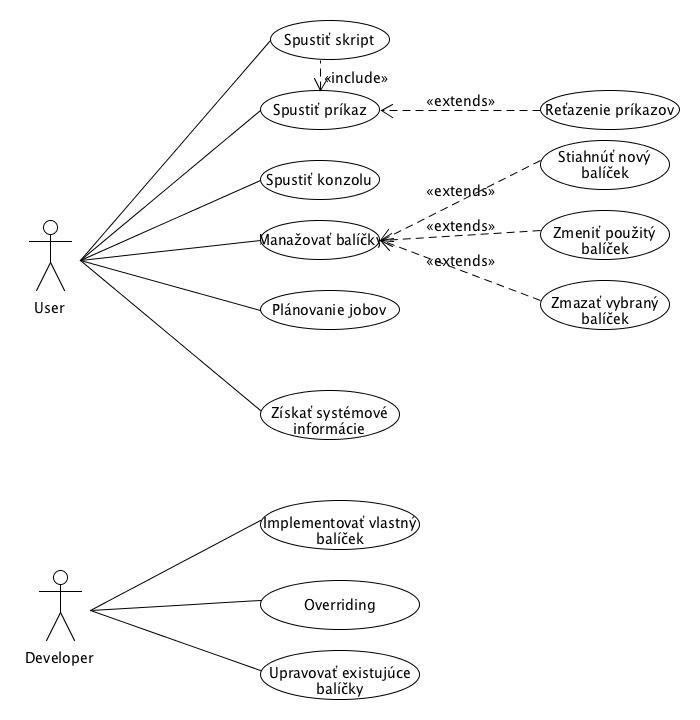
\includegraphics[width=\linewidth]{img/usecase.jpg}
	\caption{Prípady použitia pre navrhovanú aplikáciu}
	\label{fig:test}
\end{figure}
\newpage
\subsection{Popis prípadov použitia}
\indent V tejto časti sa venujeme popisu jednotlivých prípadov použitia. Diagram prípadov použitia spolu s popisom sú základnými prvkami, na ktorých je možné špecifikovať novovznikajúci softvér. Je dôležité najpodstatnejšie časti systému špecifikovať na začiatku, aby pri navrhovaní aplikácie mohli byť prijaté rozhodnutia zaručujúce dosiahnutie najlepšieho výsledného riešenia vyhovujúceho špecifikácii. Ako je zjavné aj z priloženého diagramu prípadov použitia, pre aplikáciu sme identifikovali dvoch hráčov : Vývojár skriptov a Vývojár balíčkov. Títo hráči majú jednu spoločnú črtu - pre obe platí, že hráč je vývojár. Avšak je rozdiel medzi vývojárom skriptu a vývojárom balíčkov(nových súčastí systému), čo môžeme vyčítať z popisu konkrétnych prípadov použitia.
\subsubsection{Vývojár skriptov}
\indent Rola sa zameriava hlavne na používanie hotovej aplikácie, prácu s balíčkami, vytváranie skriptov, efektívne využívanie dostupného \acrshort{api}. 
\paragraph{UC1\_Spustiť konzolu}
\begin{center}
	\begin{longtable}{|p{2.5cm}|p{12.2cm}|}
		\hline
		\textbf{Use case} & UC1\_Spustiť konzolu \\ 
		\hline
		\textbf{Podmienky} & Používateľ musí disponovať stiahnutou aplikáciou.\\
		\hline
		\textbf{Vstup} & Nie je potrebný žiadny vstup od používateľa.\\
		\hline
		\textbf{Popis} & Konzolové rozhranie sa spustí. \\ 
		\hline
		\textbf{Výstup} & Konzola zobrazí základné údaje o konfigurácii.\\
		\hline
		\textbf{Chyba} & Konzola sa nespustí, musí však poskytnúť informáciu o chybe ktorá pri štarte nastala.\\
		\hline
	\caption{Use case : Spustiť konzolu}
	\label{table:1}
	\end{longtable}
\end{center}

\paragraph{UC2\_Spustiť príkaz}
\begin{center}
	\begin{longtable}{|p{2.5cm}|p{12.2cm}|}
		\hline
		\textbf{Use case} & UC2\_Spustiť príkaz \\ 
		\hline
		\textbf{Podmienky} & Shell aplikácia musí byť spustená. \\ 
		\hline
		\textbf{Vstup} & Textový reťazec obsahujúci príkaz a jeho argumenty.\\
		\hline
		\textbf{Popis} & Používateľ zadá platný príkaz, následne získa výstup pre zadaný príkaz. \\ 
		\hline
		\textbf{Výstup} & Textový reťazec, ktorý sa v závislosti od programu mení v dĺžke a obsahu.\\
		\hline
		\textbf{Chyba} & V prípade zlyhania je používateľ informovaný o probléme, ktorý nastal.\\
		\hline
		\caption{Use case : Spustiť príkaz}
		\label{table:1}
	\end{longtable}
	
\end{center}
\paragraph{UC3\_Spustiť skript}
\begin{center}
	\begin{longtable}{|p{2.5cm}|p{12.2cm}|}
		\hline
		\textbf{Use case} & UC3\_Spustiť skript \\ 
		\hline
		\textbf{Podmienky} & Shell aplikácia musí byť spustená a skript správne napísaný.\\ 
		\hline
		\textbf{Vstup} & Vstupom je skript, definujúci v hlavičke balíčky ktoré bude používať. Za nimi môže nasledovať čokoľvek od definície premenných, funkcií. V tele skriptu musí byť zadefinovaná metóda main(String args).\\
		\hline
		\textbf{Popis} & Vykonajú sa všetky príkazy tak, ako sú napísané v zdrojovom súbore. \\ 
		\hline
		\textbf{Výstup} & Výstup je textový reťazec, závislý na logike skriptu.\\
		\hline
		\textbf{Chyba} & V prípade chyby pri sťahovaní závislostí, exekúcie príkazov alebo iných komplikácií počas behu, program zapisuje na štandardný chybový výstup chybové hlášky spolu so základným popisom problému, tracom.\\
		\hline
		\caption{Use case : Spustiť skript}
		\label{table:1}
	\end{longtable}

\end{center}

\paragraph{UC4\_Spustiť Shell príkaz}
\begin{center}
	\begin{longtable}{|p{2.5cm}|p{12.2cm}|}

			\hline
			\textbf{Use case} & UC4\_Spustiť Shell príkaz \\ 
			\hline
			\textbf{Podmienky} & Shell aplikácia musí byť spustená a skript správne napísaný. Taktiež musí byť v operačnom systéme ktorý podporuje Shell. \\ 
			\hline
			\textbf{Vstup} & Textový reťazec obsahujúci príkaz a jeho argumenty.\\
			\hline
			\textbf{Popis} & Používateľ zadá platný príkaz, následne získa výstup pre zadaný príkaz. \\ 
			\hline
			\textbf{Výstup} &Textový reťazec, ktorý sa v závislosti od programu mení v dĺžke a obsahu. \\
			\hline
			\textbf{Chyba} & V prípade zlyhania je používateľovi vratený chybový kód.\\
			\hline
		\caption{Use case : Spustiť shell príkaz}
	\label{table:1}
	
	\end{longtable}
\end{center}

\paragraph{UC5\_Spustiť commander príkaz}
\begin{center}
	\begin{longtable}{|p{2.5cm}|p{12.2cm}|}

			\hline
			\textbf{Use case} & UC5\_Spustiť commander príkaz \\ 
			\hline
			\textbf{Podmienky} & Shell aplikácia musí byť spustená a skript správne napísaný. Systém musí mať nainštalovaný Windows commander.\\ 
			\hline
			\textbf{Vstup} & Textový reťazec obsahujúci príkaz a jeho argumenty.\\
			\hline
			\textbf{Popis} & Používateľ zadá platný príkaz začinajúci win alebo ext, následne získa výstup pre zadaný príkaz. \\ 
			\hline
			\textbf{Výstup} &Textový reťazec, ktorý sa v závislosti od programu mení v dĺžke a obsahu. \\
			\hline
			\textbf{Chyba} & V prípade zlyhania je používateľovi vratený chybový výstup z príkazového riadku.\\
			\hline
	\caption{Use case : Spustiť powershell príkaz}
	\label{table:1}

	\end{longtable}
\end{center}
\paragraph{UC6\_Reťazenie príkazov}
\begin{center}
	\begin{longtable}{|p{2.5cm}|p{12.2cm}|}

			\hline
			\textbf{Use case} & UC6\_Reťazenie príkazov \\ 
			\hline
			\textbf{Podmienky} & Shell aplikácia musí byť spustená. Vstup musí byť zadaný v správnom formáte.\\ 
			\hline
			\textbf{Vstup} & Textový reťazec obsahujúci sekvenciu príkazov, ich argumenty spojené znakom pajpy "|".\\
			\hline
			\textbf{Popis} & Systém rozozná, že ide o zreťazený príkaz a následne začne vykonávať príkazy v poradí v akom boli zadané. Jednotlivé príkazy odovzdajú  výstupy nasledovníkovi po úspešnom ukončení. Príkazy sa vykonávajú dovtedy, pokým nepríde na posledný príkaz v sekvencii, alebo ak počas behu nastane chyba. O chybe je používateľ oboznámený a chyba je zapísaná na štandardný chybový výstup. \\ 
			\hline

			\textbf{Výstup} & Textový reťazec, ktorý sa v závislosti od programu mení v dĺžke a obsahu, výstup bude vygenerovaný posledným príkazom sekvencie.\\
			\hline

			\textbf{Chyba} & O chybe je používateľ oboznámený a chyba je zapísaná na štandardný chybový výstup.\\
			\hline
	\caption{Use case : Reťazie príkazov}
	\label{table:1}

	\end{longtable}
\end{center}


\paragraph{UC7\_Manažovať balíčky}
\begin{center}
	\begin{longtable}{|p{2.5cm}|p{12.2cm}|}

			\hline
			\textbf{Use case} & UC7\_Manažovať balíčky \\ 
			\hline
			\textbf{Podmienky} & Shell aplikácia musí byť spustená.\\ 
			\hline
			\textbf{Vstup} & Textový reťazec obsahujúci príkaz pkg a jeho argumenty.\\
			\hline
			\textbf{Popis} & Používateľ bude schopný nahrať, zmazať, nahradiť vybraný balíček. \\ 
			\hline
			\textbf{Výstup} & Textový reťazec, ktorý sa v závislosti od programu mení v dĺžke a obsahu .\\
			\hline
			\textbf{Chyba} & O chybe je používateľ oboznámený a chyba je zapísaná na štandardný chybový výstup.\\
			\hline
	\caption{Use case : Manažovať balíčky}
	\label{table:1}

	\end{longtable}
\end{center}
\paragraph{UC8\_Stiahnuť nový balíček}
\begin{center}
	\begin{longtable}{|p{2.5cm}|p{12.2cm}|}
			\hline
			\textbf{Use case} & UC8\_Stiahnuť nový balíček \\ 
			\hline
			\textbf{Podmienky} & Shell aplikácia musí byť spustená. Príkaz na stiahnutie balíčka musí byť správne zadaný.\\ 
			\hline
			\textbf{Vstup} & Textový reťazec obsahujúci príkaz "pkg download <názov balička s verziou>"\\
			\hline
			\textbf{Popis} & Program ako prvé skontroluje adresár balíčkov, či daný balíček nebol stiahnutý, ak nie stiahne nový balíček. V opačnom prípade medzi aktívne balíčky načíta používateľom zvolený balíček.\\ 
			\hline
			\textbf{Výstup} & Textový reťazec  informujúci o úspešnosti sťahovania. Pre jeho načítanie je potrebný reštart aplikácie.\\
			\hline

			\textbf{Chyba} & Vypíše chybu na štandardný chybový výstup v prípade, že daný balíček na servery neexistuje, používateľ nemá internetové pripojenie.\\
			\hline
		\caption{Use case : Stiahnúť nový balíček}
		\label{table:1}
		
	\end{longtable}
\end{center}

\paragraph{UC9\_Zmeniť  použitý balíček}
\begin{center}
	\begin{longtable}{|p{2.5cm}|p{12.2cm}|}
		
			\hline
			\textbf{Use case} & UC9\_Zmeniť  použitý balíček \\ 
			\hline
			\textbf{Podmienky} & Shell aplikácia musí byť spustená. Príkaz na zmenu používaného balíčka musí byť správne zadaný.\\ 
			\hline
			\textbf{Vstup} & Textový reťazec obsahujúci príkaz "pkg change  <názov nahradzujúceho balíčka s verziou>\\
			\hline
			\textbf{Popis} & Program zmení používaný balíček z aktuálne používaného na balíček vybratý používateľom. Táto voľba je aplikovateľná iba pre spravovanie verzií existujúcich balíčkov. V prípade, že nahradzujúci balíček nie je dostupný lokálne, používateľ bude vyzvaný stiahnúť daný balíček.\\ 
			\hline
			\textbf{Výstup} & Textový reťazec informujúci o úspešnosti výmeny, alebo informujúci o potrebe stiahnutia balíčka.\\
			\hline
			\textbf{Chyba} & V prípade ak dôjde počas zmeny balíčkov ku chybe, bude zapísaná na štandardný chybový výstup.\\
			\hline
		\caption{Use case : Zmeniť  použiťý balíček}
		\label{table:1}
		
	\end{longtable}
\end{center}

\paragraph{UC10\_Zmazať vybraný balíček}
\begin{center}
	\begin{longtable}{|p{2.5cm}|p{12.2cm}|}
		
			\hline
			\textbf{Use case} & UC10\_Zmazať vybraný balíček \\ 
			\hline
			\textbf{Vstup} & Textový reťazec obsahujúci príkaz "pkg delete <názov balíčka>.\\
			\hline
			\textbf{Podmienky} & Shell aplikácia musí byť spustená. Príkaz na zmazanie vybraného balíčka musí byť správne zadaný.\\ 
			\hline
			\textbf{Popis} & Program zmaže používateľom vybraný balíček z aktívnych balíčkov a následne ho fyzicky zmaže z disku. \\
			\hline

			\textbf{Výstup} & Textový reťazec informujúci o úspešnosti zmazania zadaného balíčka\\
			\hline
			\textbf{Chyba} & V prípade nesprávneho odstránenia balíčka z aktívnych balíčkov alebo pri následnom zmazaní zo súborového systému bude informácia o chybe presmerovaná na štandardný chybový výstup.\\
			\hline
		\caption{Use case : Zmazať vybraný balíček}
		\label{table:1}
		
	\end{longtable}
\end{center}
\paragraph{UC11\_Získať systémové informácie}
\begin{center}
	\begin{longtable}{|p{2.5cm}|p{12.2cm}|}
		
			\hline
			\textbf{Use case} & UC11\_Získať systémové informácie \\ 
			\hline
			\textbf{Vstup} & Vstupom je textový reťazec "sysinfo".\\
			\hline
			\textbf{Podmienky} & Shell aplikácia musí byť spustená. Používateľ vloží platný príkaz na vyžiadanie systémových informácií. \\ 
			\hline
			\textbf{Popis} & Program vypíše na štandardný výstup informácie o využití systémových zdrojov,  ako napríklad využitie procesora, využitie pamäte RAM, využitie oddielu swap a podobne.\\ 
			\hline
					
			\textbf{Výstup} & Výstupom je textový reťazec, formátovaný do riadkov. Každému riadku prislúcha jedna informácia, napr. CPU, ďalší riadok RAM atď.. V prípade viac jadrového procesora sa vypíšu informácie o každom z jadier.  \\
			\hline
			\textbf{Chyba} & V prípade, že používateľ nemá právo na získanie informácií, program vypíše dôvod priamo na štandardný výstup. Rovnako program vypíše aj akékoľvek chyby, ku ktorým môže dôjsť počas behu.\\
			\hline
		\caption{Use case : Získať systémové informácie}
		\label{table:1}
		
	\end{longtable}
\end{center}

\paragraph{UC12\_Získať informácie o procesoch}
\begin{center}
	\begin{longtable}{|p{2.5cm}|p{12.2cm}|}
		
			\hline
			\textbf{Use case} & UC12\_Získať informácie o procesoch \\ 
			\hline
			\textbf{Vstup} & Vstupom je textový reťazec "processes".\\
			\hline
			\textbf{Podmienky} & Shell aplikácia musí byť spustená. Používateľ vloží platný príkaz na vyžiadanie informácií o procesoch. \\ 
			\hline

			\textbf{Popis} & Program vypíše na štandardný výstup informácie o spustených procesoch, používateľoch, ktorí tieto procesy spúšťajú, koľko percent procesoru, pamäte RAM používajú.\\ 
			\hline

			\textbf{Výstup} & Výstupom je prehľadný výpis v podobe tabuľky, kde každý riadok zodpovedá jednému procesu. Nad jednotlivými hodnotami je hlavný riadok, ktorý popisuje o akú hodnotu ide.\\
			\hline
			\textbf{Chyba} & V prípade, že nie je možné získať informácie o procesoch, je táto skutočnosť zobrazená na stdout a popis chyby sa presmeruje na štandardný chybový výstup.\\
			\hline
		\caption{Use case : Získať informácie o procesoch}
		\label{table:1}
		
	\end{longtable}
\end{center}
\paragraph{UC13\_Vytvoriť skript}
\begin{center}
	\begin{longtable}{|p{2.5cm}|p{12.2cm}|}
		
			\hline
			\textbf{Use case} & UC13\_Vytvoriť skript \\ 
			\hline
			\textbf{Podmienky} & Používateľ musí mať prístup k akémukoľvek textovému editoru.  \\ 
			\hline
			\textbf{Vstup} & Vstupom musí byť správne napísaný skript. \\
			\hline
			\textbf{Popis} & Používateľ napíše skrip, ktorý bude prečítaný programom a vykonaný.\\ 
			\hline
			\textbf{Výstup} & Skrip vráti výstup svojho beho buď na štandardný výstup, alebo do súboru, v závislosti od toho ako je naimplementovaný.\\
			\hline
			\textbf{Chyba} & V prípade, že dôjde k menšej chybe, informácia bude zobrazená používateľovi, resp. presmerovaná do súboru.\\
			\hline
		\caption{Use case : Vytvoriť skript}
		\label{table:1}
		
	\end{longtable}
\end{center}
\paragraph{UC14\_Vytvoriť funkciu}
\begin{center}
	\begin{longtable}{|p{2.5cm}|p{12.2cm}|}
		
			\hline
			\textbf{Use case} & UC14\_Vytvoriť funkciu \\ 
			\hline
			\textbf{Podmienky} & Používateľ musí mať prístup k akémukoľvek textovému editoru.  \\ 
			\hline
			\textbf{Vstup} & Funkcia musí byť správne zadefinovaná. 
			Syntax pre definovanie funkcie : 
			\newline
			function <návratový typ> <názov funkcie>(parametre funkcie){telo funkcie}. \\
			\hline
			
			\textbf{Popis} & Používateľ napíše funkciu, ktorá bude prečítaná programom a vykonaná.\\ 
			\hline

			\textbf{Výstup} & Funkcia vracia premennú s definovanou návratovou hodnotou.\\
			\hline
			\textbf{Chyba} & V prípade, že nastane chyba pri exekúcii funkcie, program skončí a zapíše informácie o chybe na štandardný chybový výstup.\\
			\hline
		\caption{Use case : Vytvoriť funkciu}
		\label{table:1}
		
	\end{longtable}
\end{center}
\paragraph{UC15\_Override funkcie}
\begin{center}
	\begin{longtable}{|p{2.5cm}|p{12.2cm}|}
		
			\hline
			\textbf{Use case} & UC15\_Override funkcie \\ 
			\hline
			\textbf{Podmienky} & Používateľ musí mať prístup k akémukoľvek textovému editoru.  \\ 
			\hline
			\textbf{Vstup} & Nad funkciou je potrebné zapísať @Override,  čo prekladaču povie, že má používať práve túto verziu funkcie.\\
			\hline
			
			\textbf{Popis} & Používateľ napíše funkciu, ktorá bude prečítaná programom a vykonaná. Navyše bude nahrádzať funkciu s rovnakým názvom.\\ 
			\hline
			\textbf{Výstup} & Premenná, ktorá je uvedená v definícii funkcie.\\
			\hline
			\textbf{Chyba} & V prípade zle zadefinovanej syntaxe je problém zapísaný na štandardný chybový výstup a vykonávanie skriptu je ukončené.\\
			\hline
		\caption{Use case : Override funkcie}
		\label{table:1}
		
	\end{longtable}
\end{center}
\paragraph{UC16\_Vytvoriť cyklus}
\begin{center}
	\begin{longtable}{|p{2.5cm}|p{12.2cm}|}
		
			\hline
			\textbf{Use case} & UC16\_Vytvoriť cyklus \\ 
			\hline
			\textbf{Podmienky} & Používateľ musí mať prístup k akémukoľvek textovému editoru.  \\ 
			\hline
			\textbf{Vstup} & Cyklus musí byť správne zadefinovaný. 
			Syntax pre definovanie funkcie : 
			\newline
			for(<inicializácia premennej>;<podmienka pre spustenie>;<inkrement>){telo cyklu obsahujúce volania funkcií, príkazy, atď..}. \\
			\hline

			\textbf{Popis} & Používateľ napíše cyklus, ktorý bude prečítaný programom a vykonaná sa.\\ 
			\hline
			\textbf{Výstup} & Cyklus nemá žiadny výstup.\\
			\hline
			\textbf{Chyba} & V prípade, že nastane chyba pri parsovaní alebo exekúcii cyklu, program skončí a zapíše informácie o chybe na štandardný chybový výstup.\\
			\hline
		\caption{Use case : Vytvoriť cyklus}
		\label{table:1}
		
	\end{longtable}
\end{center}
\paragraph{UC17\_Vytvoriť podmienku}
\begin{center}
	\begin{longtable}{|p{2.5cm}|p{12.2cm}|}
		
			\hline
			\textbf{Use case} & UC17\_Vytvoriť podmienku \\ 
			\hline
			\textbf{Podmienky} & Používateľ musí mať prístup k akémukoľvek textovému editoru.  \\ 
			\hline
			\textbf{Vstup} & Podmienka musí byť správne zadefinovaná. 
			Syntax pre definovanie podmienky : 
			\newline
			if(boolean value){telo podmienky obsahujúce volania funkcií, príkazy, atď..}. \\
			\hline
			\textbf{Popis} & Používateľ napíše podmienku, ktorá bude prečítaná programom a zohľadnená počas behu skriptu.\\ 
			\hline
			\textbf{Výstup} & Podmienka nemá žiadny výstup.\\
			\hline
			\textbf{Chyba} & V prípade, že nastane chyba pri parsovaní alebo exekúcii podmienky, program skončí a zapíše informácie o chybe na štandardný chybový výstup.\\
			\hline
		\caption{Use case : Vytvoriť podmienku}
		\label{table:1}
		
	\end{longtable}
\end{center}
\paragraph{UC18\_Vytvoriť premenné}
\begin{center}
	\begin{longtable}{|p{2.5cm}|p{12.2cm}|}
		
			\hline
			\textbf{Use case} & UC18\_Vytvoriť premenné \\ 
			\hline
			\textbf{Podmienky} & Používateľ musí mať prístup k akémukoľvek textovému editoru.  \\ 
			\hline
			\textbf{Vstup} & Premenná musí byť správne zadefinovaná. 
			\newline
			Syntax pre definovanie premennej : 
			\newline
			<typ> <názov premennej>; alebo 
			\newline
			 <typ> <názov premennej> = <hodnota>;
			 \newline
			 , kde hodnota môže byť konkrétna hodnota alebo iná premenná rovnakého typu.\\
			\hline
			\textbf{Popis} & Používateľ napíše inicializáciu alebo definíciu premennej, ktorá bude prečítaná programom a vykonaná.\\ 
			\hline
			\textbf{Výstup} & Program si uloží premmenú a jej hodnotu, ak bola definovaná.\\
			\hline
			\textbf{Chyba} & V prípade, že nastane chyba, používateľ bude informovaný o neúspechu na štandardný chybový výstup.\\
			\hline
			\caption{Use case : Vytvoriť premenné}
		\label{table:1}
	
	\end{longtable}
\end{center}
\paragraph{UC19\_Vykonať základné aritmetické operácie}
\begin{center}
	\begin{longtable}{|p{2.5cm}|p{12.2cm}|}
		
			\hline
			\textbf{Use case} & UC19\_Vykonať základné aritmetické operácie \\ 
			\hline
			\textbf{Podmienky} & Používateľ musí mať prístup k akémukoľvek textovému editoru.  \\ 
			\hline
			\textbf{Vstup} & Premenná musí byť správne zadefinovaná. 
			\newline
			Syntax pre definovanie /zmenu hodnoty premennej: 
			\newline
			<názov premennej> = <výraz>; alebo 
			\newline
			<typ> <názov premennej> = <výraz>;
			\newline
			, kde výraz môže byť operácia nad číselnými hodnotami a číselnými premennými. \\
			\hline
			\textbf{Popis} & Používateľ napíše príkaz, ktorý bude prečítaný programom a vykonaný.\\ 
			\hline
			\textbf{Výstup} & Príkaz nastaví hodnotu premennej s vypočítanou návratovou hodnotou.\\
			\hline
			\textbf{Chyba} & V prípade, že nastane chyba pri exekúcii príkazu, program skončí a zapíše informácie o chybe na štandardný chybový výstup.\\
			\hline
		\caption{Use case : Vytvoriť funkciu}
		\label{table:1}
		
	\end{longtable}
\end{center}
\paragraph{UC20\_Vykonať základné logické operácie}
\begin{center}
	\begin{longtable}{|p{2.5cm}|p{12.2cm}|}
		
			\hline
			\textbf{Use case} & UC20\_Vykonať základné logické operácie\\ 
			\hline
			\textbf{Podmienky} & Používateľ musí mať prístup k akémukoľvek textovému editoru.  \\ 
			\hline
			\textbf{Vstup} & Premenná musí byť správne zadefinovaná. \newline
			Syntax pre definovanie /zmenu hodnoty premennej:  \newline
			<názov premennej> = <výraz>; alebo \newline
			<typ> <názov premennej> = <výraz>;
			\newline
			, kde výraz môže byť operácia nad číselnými hodnotami, číselnými premennými, ako aj nad pravdivostnými.\newline
			Vzťahy medzi číselnými hodnotami musia byť definované logickými operátormi - <, >, <=, >=, ==, !=.\newline
			Vzťahy medzi pravdivostnými hodnotami musia byť definované logickými operátormi : ==, !=, ||, \&\&.  \\
			\hline
			\textbf{Popis} & Používateľ napíše príkaz, ktorý bude prečítaný programom a vykonaný.\\ 
			\hline
			\textbf{Výstup} & Príkaz nastaví hodnotu premennej s vypočítanou návratovou hodnotou.\\
			\hline
			\textbf{Chyba} & V prípade, že nastane chyba pri exekúcii príkazu, program skončí a zapíše informácie o chybe na štandardný chybový výstup.\\
			\hline
		\caption{Use case : Vytvoriť funkciu}
		\label{table:1}
		
	\end{longtable}
\end{center}

\paragraph{UC21\_Presmerovať chybový výstup}
\begin{center}
	\begin{longtable}{|p{2.5cm}|p{12.2cm}|}
		
			\hline
			\textbf{Use case} & UC21\_Presmerovať chybový výstup \\ 
			\hline
			\textbf{Vstup} & Pre presmerovanie na chybový výstup je potrebné dodržať syntax command stderr> file\\
			\hline
			\textbf{Podmienky} & Shell aplikácia musí byť spustená. Používateľ vloží platný príkaz na presmerovanie chybového výstupu. \\ 
			\hline
			\textbf{Popis} & Program presmeruje chybový výstup tam, kam mu používateľ v príkaze zadefinuje. \\ 
			\hline
			\textbf{Výstup} & Výstup programu predstavuje textový reťazec s popisom chyby, ktorá nastala.\\
			\hline
			\textbf{Chyba} & Ak by došlo ku chybe, chyba sa zapíše sa do logu aplikácie.\\
			\hline
		\caption{Use case : Presmerovať chybový výstup}
		\label{table:1}
		
	\end{longtable}
\end{center}
\paragraph{UC22\_Presmerovať štandardný výstup}
\begin{center}
	\begin{longtable}{|p{2.5cm}|p{12.2cm}|}
		
			\hline
			\textbf{Use case} & UC22\_Presmerovať štandardný výstup \\ 
			\hline
			\textbf{Podmienky} & Shell aplikácia musí byť spustená. Používateľ vloží platný príkaz na presmerovanie štandardného výstupu. \\ 
			\hline
			\textbf{Vstup} & Pre presmerovanie na štandardný výstup je potrebné dodržať syntax command stdout> file\\
			\hline
			\textbf{Popis} & Program presmeruje štandardný výstup tam, kam mu používateľ v príkaze zadefinuje.\\ 
			\hline
			\textbf{Výstup} & Výstup programu predstavuje textový reťazec s výstupom zo skriptu alebo príkazu.\\
			\hline
			\textbf{Chyba} & Ak by došlo ku chybe, chyba sa zapíše sa do logu aplikácie.\\
			\hline
		\caption{Use case : Presmerovať štandardný výstup }
		\label{table:1}
		
	\end{longtable}
\end{center}



\subsubsection{Vývojár balíčkov}
\indent Vychádzajúc z názvu role je zjavné, že tento hráč sa bude starať o vývoj aplikácie a jej funkcionalitu v zmysle rozširovania \acrshort{api}, ktoré môže vývojár skriptov používať pre efektívnejšiu prácu.
\paragraph{UC23\_Implementovať vlastný balíček}
\begin{center}
	\begin{longtable}{|p{2.5cm}|p{12.2cm}|}
		
			\hline
			\textbf{Use case} & UC23\_Implementovať vlastný balíček \\ 
			\hline
			\textbf{Podmienky} & Používateľ musí mať nainštalovanú Java SDK vo verzii 8, mať prístup k textovému editoru.  \\ 
			\hline
			\textbf{Vstup} & Balíček obsahujúci všetky potrebné rozhrania, ktoré musí vývojár balíčka implementovať.\\
			\hline
			\textbf{Popis} & Používateľ implementuje novú funkcionalitu v Jave, následne všetky zdrojové súbory skompiluje a pridá do \acrshort{jar} súboru určeného na ukladanie nových balíčkov.\\ 
			\hline
			\textbf{Výstup} & Balíček, ktorý je možné nahrať do aplikácie a používať ako jeden z príkazov.\\
			\hline
			\textbf{Chyba} & Chyba môže nastať pri vytváraní balíčka, kedy vývojára o chybe informuje prekladač jazyka, v ktorom je balíček implementovaný. V prípade neúspešného načítania je používateľ informovaný priamo v konzole na štandardný výstup.\\
			\hline
		\caption{Use case : Implementovať vlastný balíček}
		\label{table:1}
		
	\end{longtable}
\end{center}

\paragraph{UC24\_Upravovať existujúce balíčky}
\begin{center}
	\begin{longtable}{|p{2.5cm}|p{12.2cm}|}
		
			\hline
			\textbf{Use case} & UC24\_Upravovať existujúce balíčky \\ 
			\hline
			\textbf{Podmienky} &  Používateľ musí mať nainštalovanú Java SDK vo verzii 8, mať prístup k textovému editoru.  \\ 
			\hline
			\textbf{Vstup} & Zdrojové súbory už existujúceho balíčka.\\
			\hline
			\textbf{Popis} & Používateľ upraví implementáciu alebo pridá novú funkcionalitu v Jave, následne všetky zdrojové súbory skompiluje a pridá do \acrshort{jar} súboru určeného na ukladanie nových balíčkov\\ 
			\hline
			\textbf{Výstup} & Po úprave je balíček možné nahrať do aplikácie a používať ako jeden z príkazov.\\
			\hline
			\textbf{Chyba} & Chyba môže nastať pri vytváraní balíčka, kedy vývojára o chybe informuje prekladač jazyka, v ktorom je balíček implementovaný. V prípade neúspešného načítania je používateľ informovaný priamo v konzole na štandardný výstup.\\
			\hline
		\caption{Use case : Upravovať existujúce balíčky}
		\label{table:1}
		
	\end{longtable}
\end{center}
\subsection{Výber programovacieho jazyka}
\indent Java je programovací jazyk a výpočtová platforma, ktorá bola vydaná spoločnosťou Sun Microsystems v roku 1995. \cite{java} 
Programy v Jave sú prvotne preložené do tzv. byte-code, ktorý je rovnaký pre všetky \acrshort{pc}. Pomocou jednoduchého programu je byte-code preložený do jazyka, ktorému rozumie konrétny \acrshort{pc}.
Java je objektovo-orientovaný programovací jazyk, čo znamená že rovnako ako v živote, aj v Jave je všetko tvorené objektami. Obsahuje široké spektrum knižníc, ktoré slúžia nielen na vývoj webových, ale aj desktopových aplikácií.
Podporuje multitrading, čo umožňuje vytvárať efektívne programy pre počítače s viacjadrovým procesorom.\cite{javabook}
\subsection{Návrhové vzory}
\indent Návrhové vzory sú všeobecne opakovaným riešním pre všeobecne opakujúci sa problém pri dizajnovaní softwéru. Návrhový vzor nie je nemenný dizajn, vždy je potrebné aby si ho programátori uspôsobili podľa vlstných potrieb. Návrhové vzory sa delia do troch základných skupín vytváracie vzory, štrukturálne vzory a vzory správania. \cite{designpattern}

\subsubsection{Factory - továreň}
\indent Factory návrhový vzor patrí do sekcie vytváracích vzorov, pomocou tohoto vzoru budeme schopný vytvárať objekty bez toho aby sme prezradili logiku ich vytvárania klientovi.\cite{designpattern}
Diagram návrhového vzoru je mozné vidieť na nasledujúcom obrázku.
\begin{figure}[!htbp]
	\centering
	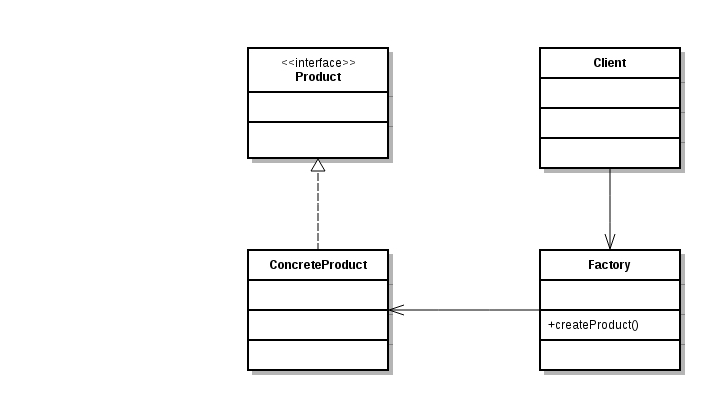
\includegraphics[width=10cm]{img/factory_design_pattern.jpg}
	\caption{Class diagram Factory návrhového vzoru}
	\label{fig:test}
\end{figure}
\newline
\subsubsection{Command - príkaz}
\indent Command pattern je známy behaviorálny návrhový vzor, používa sa najmä na menežovanie algoritmov, vzťahov a zodpovednosti medzi objektami. 
Cieľom vzoru je zapúzdriť požiadavku(request) ako objekt tým pádom parametrizovať klienta s rôznymi požiadavkami a zabezpečiť operáciu spať.\cite{designpattern}
\begin{figure}[!htbp]
	\centering
	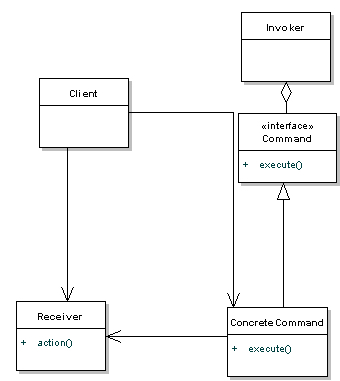
\includegraphics[width=10cm]{img/command_pattern_class.jpg}
	\caption{Class diagram Command návrhového vzoru}
	\label{fig:test}
\end{figure}
\newline
Command vzor deklaruje rozhranie pre všetky budúce commandy a zároveň execute() metódu, ktorú s vypýta Receiver commandu aby splnil požadovanú operáciu.
Receiver je objekt, ktorý vie ako požadovanú operáciu splniť. Invoker pozná command a pomocou implementovanej execute() metódy dokáže vyvolať požadovanú operáciu.
Klient potrebuje implemenotvaž ConcreteCommand a nastavit Receiver pre command. ConcreteCommand definuje spojenie medzi action a receiver. Keď Invoker zavolá execute() metódu na ConcreteCommand spustí tým jednu alebo viac akcií, ktoré budú bežať pomocou Receivera.\cite{designpattern}

Pre lepšie pochopenie je proces zobrazený aj na sekvenčnom diagrame.
\begin{figure}[!htbp]
	\centering
	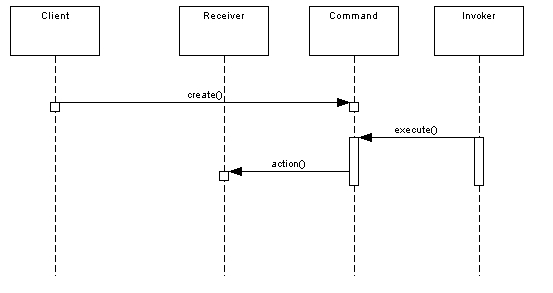
\includegraphics[width=10cm]{img/command_seq.jpg}
	\caption{Sekvenčný diagram Command návrhového vzoru}
	\label{fig:test}
\end{figure}
\newline

\subsection{Aplikácia}
\indent Pre implementáciu vlastného riešenia bolo potrebné na základe prípadov použitia identifikovať časti, z ktorých bude aplikácia pozostávať. Naším zámerom nebolo vytvorenie jednej veľkej aplikácie, ktorá by sa mohla časom stať neudržiavateľnou, ale aplikácia, ktorá umožní používateľom interaktívny aj skriptovací módus. Rozhodli sme sa, že navrhneme jednu hlavnú aplikáciu, ktorá bude mať na starosti interaktívny prístup pre používateľa rovnako aj skriptovací módus, avšak funkcionality, ktoré bude podporovať, zabezpečia menšie externé podprogrami - pluginy, ktoré sa do apikácie nahrajú pri štarte. Pre dosiahnutie požadovaných výsledkov použijeme návrhový vzor Command. Ako ďalšie sme definovali komponenty aplikácie.

\subsection{Komponenty aplikácie}
\indent Po vybratí návrhového vzoru sme prešli na identifikáciu komponentov aplikácie. V prvom návrhu sme identifikovali niekoľko komponentov, ktoré považujeme za podstatné a potrebné pre správny chod programu. Z týchto komponentov sme následne vytvorili malý projekt, kde sme sa pokúsili vytvoriť niekoľko pluginov implementovaných pomocou command dizajnového návrhu na demonštrovanie funkčnosti. Nakoľko bol model funkčný, rozhodli sme sa pokračovať s jeho vývojom. Uvádzame aj komponenty, ktoré sme identifikovali pri vytváraní tejto ukážky funkčnosti : 
\begin{itemize}
	\item Parser - vstupov aj výstupov,
	\item Loader - na nahrávanie  \acrshort{jar} súborov,
	\item Sťahovač závislostí - \acrshort{jar} súbory, ktoré momentálne produkt neobsahuje napr. vlastné riešenia,
	\item Scope - je oblasť kde sa definujú premenné, funkcie a pod., tento komponent slúži na vytváranie scopov v rámci aplikácie,
	\item ScopeData - ktoré majú slúžiť na udržovanie dát v jednotlivých scopoch,
	\item ShellPlugin - komponent, ktorý nesie implementáciu príkazov.
\end{itemize}

 \begin{figure}[!htbp]
	\centering
	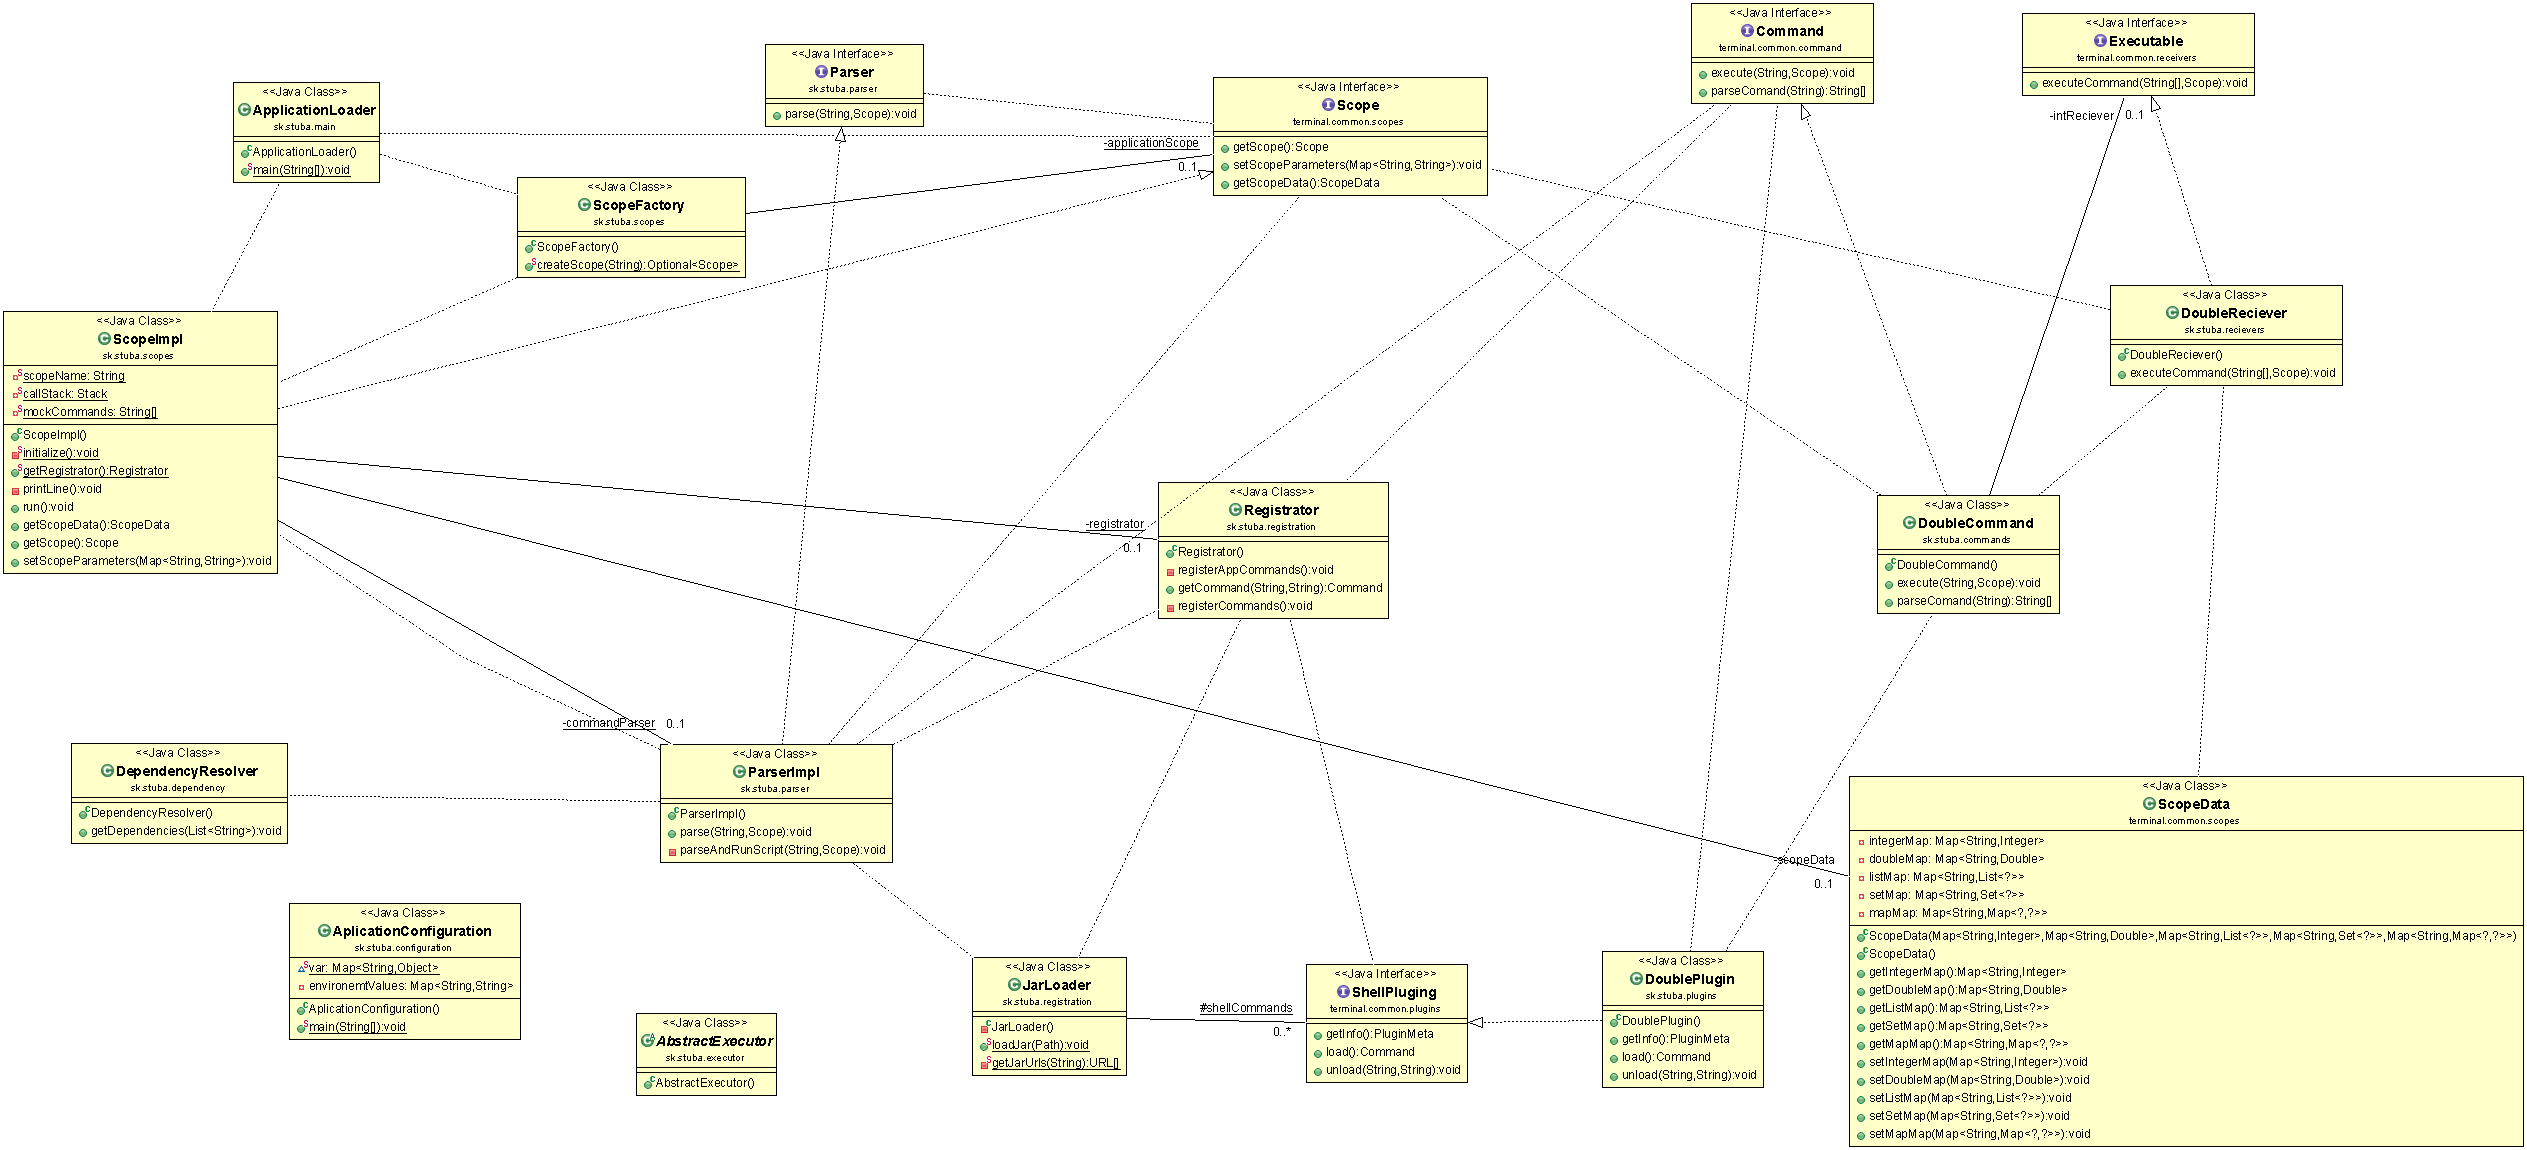
\includegraphics[width=\linewidth]{img/first_attemp_class_diag.jpg}
	\caption{Pvrvé funkčné riešenie}
	\label{fig:test}
\end{figure}
\newline
\subsection{Plugin}
\indent Z nasledovného diagramu tried nebolo na prvý pohľad zjavné aké komponenty v programe existujú, preto bolo potrebné tieto komponenty rozumne rodeliť. Z prvotného návrhu sme vytiahli plugin, ktorý bude slúžiť na nahrávanie nových funkcionalít do programu.  Diagram implementácie rozhraní a konkrétnych tried  je viditeľný na nasledovnom obrázku. 
\newpage
 \begin{figure}[!htbp]
	\centering
	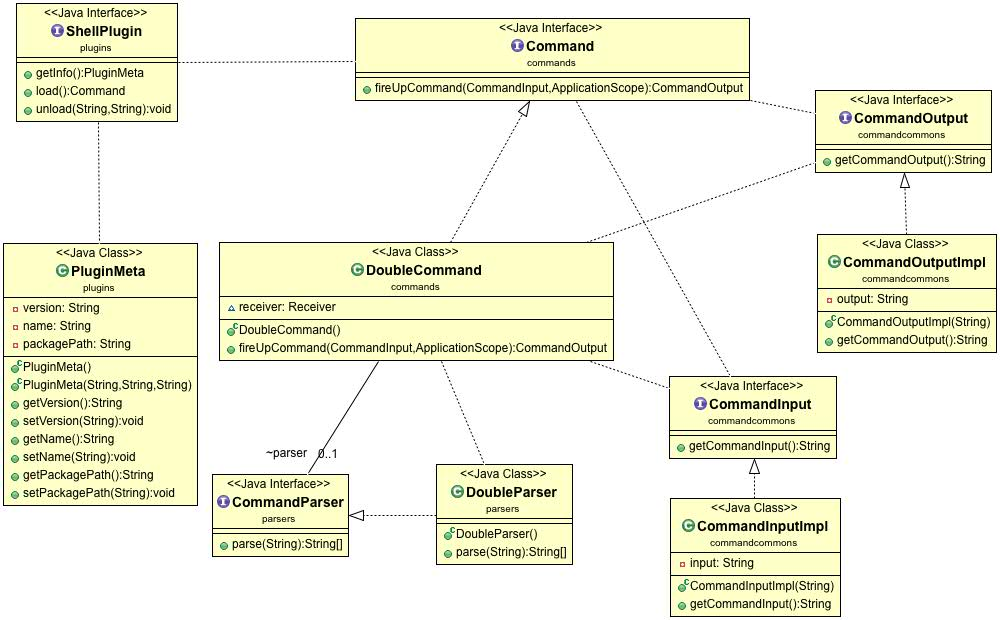
\includegraphics[width=\linewidth]{img/plugin_class.jpg}
	\caption{Plugin - diagram tried}
	\label{fig:test}
\end{figure}
\newline
\indent Ako vidieť z diagramu, Plugin pozostáva z nasledovných častí :
\begin{itemize}
	\item ShellPlugin - je rozhranie, ktoré slúži na získavanie inštancií commandu, ako aj informáciách o plugine, 
	\item Command - rozhranie, slúžiace na komunikáciu s receivermi,
	\item Receiver - triedy, ktoré implementujú receiver špecifikujú funkcionalitu pluginu,
	\item CommandParser - obsahuje parser vstupov,
	\item CommandOutput - rozhranie pre výstupy z commandu,
	\item CommandInput - rozhranie pre vstupy z commandu,
	\item  PluginMeta - nesie základné informácie o plugine.
\end{itemize}
Aj keď náš prvotý program fungoval správne čakali sme, že počas vývoja ešte môže dôjsť k obmenám tried a rozhraní, nakoľko málokedy sa podarí odhadnúť  všetky kľúčové časti už počas návrhu.

\newpage
\subsection{Diagram tried aplikácie}
 \begin{figure}[!htbp]
	\centering
	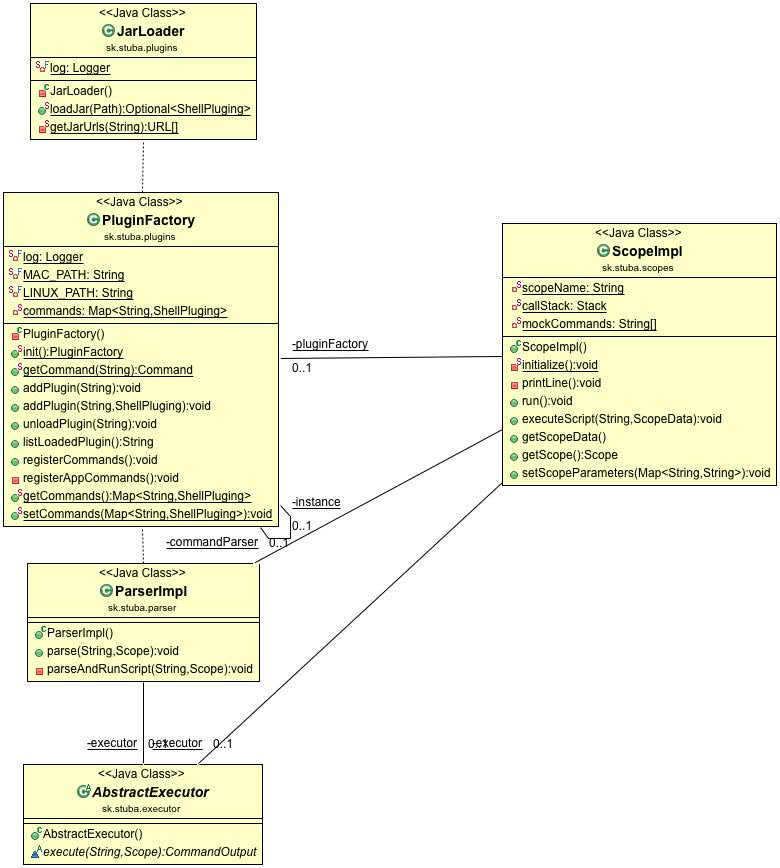
\includegraphics[scale=0.4]{img/ClassApplication.jpg}
	\caption{Diagram tried aplikácie}
	\label{fig:test}
\end{figure}
\subsubsection{Stručný popis tried}
\indent Obrázok 16 zobrazuje diagram tried aplikácie, ktoré v nasledujúcej časti stručne predstavíme.
\paragraph{ScopeImpl}
Táto trieda je jednou z najhlavnejších celého programu, tvorí základný pilier pre tvorbu akýchkoľvek scopov aplikácie, beh skriptov a pochopiteľne príkazov v interaktívnom móde. Obsahuje informácie o všetkých pluginoch, ktoré sa nahrali pri štarte aplikácie, názov scopu a inštanciu exekútora, pomocou ktorého sa vykonávajú všetky operácie v aplikácii. Implementuje metódy run() pre zabezpečenie interaktívneho módu, kde sa však môžu spúšťať aj skripty. Tiež implementuje metódu executeScript(String function, ScopeData scopeData), ktorá slúži na rekurzívne volanie funkcií v skriptovacom móde a  spúšťanie ich príkazov.
\paragraph{AbstractExecutor}
Trieda AbstractExecutor je abstraktná trieda poskytujúca abstraktnú metódu,  CommandOutput execute(String command, Scope scope). Vstupom do tejto metódy je príkaz od používateľa a scope v ktorom ho chce vykonať. Definovanie scopu nám slúži na informovanie jednotlivých prijímačov(Reciever), kde sa má daný príkaz vykonať. Ak by scope nebol presne definovaný, aplikácia by sa nevedela rozhodnúť kde sa majú príkazy premietnuť a vyhodila by chybu.
\paragraph{ParserImpl}
RootParser je najpodstatnejšia trieda pre skriptovací mód. Jej úlohou je načítať zdrojové súbory skriptu a následne spustiť exekúciu, ak parsovanie prebehlo v poriadku.
\paragraph{PluginFactory}
PluginFactory, ako z jej názvu vyplýva, je továreň, do ktorej sa pri štarte aplikácie nahrávajú všetky pluginy dostupné z disku. Na získavanie dostupných pluginov sa používa trieda JarLoader. 
\paragraph{JarLoader}
JarLoade je trieda, ktorá pomocou class loadera nahráva nové pluginy do aplikácie.
\section{Implementácia}
\indent V tejto kapitole sa budeme venovať konkrétnemu riešeniu problematiky jednotnej platformy určenej na vytváranie skrípt. Kapitola postupne definuje jednotlivé kroky implementácie riešenia. Každý krok je popísaný jednou z nasledovných možností alebo ich kombináciou: pomocou diagramu aktivít, diagramu tried, pseudokódom, prípadne útržkami zdrojového kódu z fungujúcej aplikácie. Jednotlivé sekcie práce sme rozdelili na základe toho, akými smermi sa môže aplikácia uberať. Rozhrania, ktoré aplikácia používa, sú uvedené v prílohe C.
\subsection{Hlavná trieda aplikácie - AbstractScope}
Táto trieda je jednou z najhlavnejších celého programu, tvorí základný pilier pre tvorbu akýchkoľvek scopov aplikácie, beh skriptov, ako aj príkazov v interaktívnom móde. Obsahuje informácie o všetkých pluginoch, ktoré sa nahrali pri štarte aplikácie, názov scopu a inštanciu exekútora, pomocou ktorého sa vykonávajú všetky operácie v aplikácii. Trieda má tiež informácie o vstupných parametroch, výstupných hodnotách a funkciách, ktoré sú v danom scope definované. Spomenuté hodnoty sa využívajú pri vytváraní a behu skriptov pre vstupné parametre funkcií, ako aj ich návratová hodnota. Implementuje rozhrania Scope, Runnable. Implementuje metódy run() pre zabezpečenie interaktívneho módu, kde sa však môžu spúšťať aj skripty. Tiež implementuje metódu executeScript(String function, ScopeVariables scopeVariables), ktorá slúži na rekurzívne volanie funkcií v skriptovacom móde a spúšťanie ich príkazov.
Implementuje funkciu runInputCommands(), pomocou ktorej je aplikácia spustená ak má na vstupe akékoľvek vstupné parametre. Túto funkcionalitu sme pridali z dôvodu integrácie s inými aplikáciami. 
\subsubsection{run}
\indent Táto metóda sa volá iba raz a to po štarte aplikácie. V cykle od používateľa získava vstupy, ktoré sa následne pokúša vykonať. Ak aplikácia nedokáže príkaz vykonať, vypíše chybu do konzoly.
\subsubsection{executeScript}
\indent Je funkcia, pomocou ktorej sa spúšta beh jednotlivých funkcií skriptu. Je definovaná všeobecne pre akýkoľvek scope, samozrejme v prípade, ak novému scopu rozsah metódy nepostačuje je potrebné ju prepísať v triede, ktorá je odvodená od AbstractScope. Základný algoritmus pre beh skriptov je opísaný v nižšie priloženom pseudokóde.
\begin{algorithm}[H]
	\begin{minted}[]{java}
	executeScript(String function, ScopeVariables scopeVariables) {
	executeGlobalCommands();
	fName = getFunctionName();
	Scope parent =  this.getParent();
	
	Scope functionScope = parent.functions.get(fName);
	setFunctionscopeVariables(scopeVariables.clone());
	
	for (String command : functionScope.stack) {
	if (command.startsWith("$(")) {
	out = executor.execute(command, functionScope);
	if (command.contains("returnValue = ")) {
	setReturnValue();
	}else{
	writeOutputs(out);
	}
	} else if (command.startsWith("fcall ")) {
	if(functionHasReturnValue(command)){
	setCallParameters();
	executeScript(function, getVariables());
	getReturnValue();
	}else{
	executeScript(function, getVariables());
	}
	}
	}
	\end{minted}
	\caption{Pseudokód všeobecnej implementácie spúšťania funkcií}
	\label{alg:gen}
\end{algorithm}
\subsubsection{ForScope}
\indent For cyklus má oproti hlavnému scopu pár rozdielov. Ako prvé si môžeme všimúť, že For scope si kopíruje referenciu premenných scopu, naopak funkcie si vytvárali hlbokú kópiu, aby sa zmeny v rôznych funkciách nepremietli do pôvodných. Zmeny sa vo funkciách dajú aplikovať iba pomocou vracania hodnôt z funkcií. Ďalšia vec navyše je cyklus v ktorom je vnorený rovnaký For cyklus ako v AbstractScope abšak obohatený o funkciu break, ako je možné vidieť v nasledujúcom kóde :
\begin{algorithm}[H]
	\begin{minted}[]{java}
	setScopeVariables(scopeVariables);
for (int i = getStart(); evalueateCondition(); i = evalueateIncremet()) {
  // for cyklus z abstract scopu obohatený o break
}

	\end{minted}
	\caption{Kód implementácie spúšťania funkcie For}
	\label{alg:gen}
\end{algorithm}
\indent Cyklus je tam pridaný aby sme dokázali evaluovať vstupy zadané v skripte. Ako prvé sa do premennej i nainicializuje výsledok exekúcie príkazu zo skriptu. Následne sa rovnakým spôsobom vyhodnotí podmienka a ak je všetko ok For cyklus sa začne vykonávať. Následne sa rovnako ako v predchádzajúcom prípade preiteruje cez celý stack For cyklu. Momentálnou limitáciou tohoto prístupu je možnosť inicializovať a iterovať iba cez premenné numerického typu. Avšak v budúcnosti je tento koncept ľahko rozšíriteľny aj pre premenné iných typov. For cyklus obsahuje tiež príkaz break, ktorý je bežnou súčasťou tejto štruktúry.
\subsubsection{IfScope}
\indent If scope je jednoduchšou implementáciou scopu ako bol For, nakoľko neobsahuje ďalšie cykly iba podmienku, ktorá ak sa vyhodnotí ako pravdivá, vykoná sa aj stack, ktorý if scope obsahuje. Na evaluáciu podmienok, priraďovanie hodnôt premenným ako aj iteráciu boli použité nami vopred naimplementované pluginy, ktoré dokážu pracovať s primitívnymi premennými Javy. 
\begin{algorithm}[H]
	\begin{minted}[]{java}
	if (evalueateCondition()) {
	  // For cyklus z abstract scopu obohatený o break
	}
	\end{minted}
	\caption{Kód implementácie spúšťania funkcie For}
	\label{alg:gen}
\end{algorithm}
\subsection{Štart aplikácie}
\indent  Na nasledujúcom obrázku je zobrazená aktivita spustenia konzoly. Ako vidieť z diagramu, aplikácia sa najprv nainicializuje, čo vysvetlíme v sekcii 4.3. Po inicializácii premenných sa vytvorí inštancia triedy ScopeImpl, ktorá je implementáciou AbstractScope triedy, charakterizovaná v predchádzajúcej sekcii práce. V ďalšom kroku aplikácia overí, či má na vstupe parametre. V prípade, ak áno vykoná ich, inak spustí konzolu, ktorá čaká na vstup od používateľa. V tejto časti popíšeme čo sa deje v prvom prípade, a teda že máme zadané parametre. 
\begin{figure}[!htbp]
	\centering
	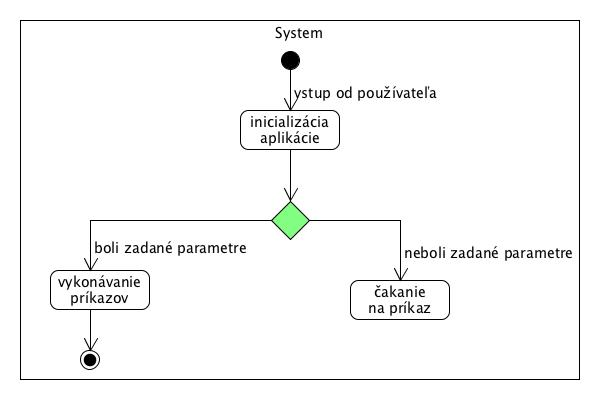
\includegraphics[width=\linewidth]{img/System.jpg}
	\caption{Activita spustenia aplikácie}
	\label{fig:test}
\end{figure}
\subsubsection{Štart s parametrami}
\indent Možnosť s parametrami na vstupe sme implementovali z dôvodu aby sa aplikácia dala integrovať s inými enterprise aplikáciami, ktoré môžu buď čítať výstupy priamo z konzoly, alebo ich môžu presmerovať do súboru. Novovytvorený súbor je následne možné načítať a vykonať nad ním potrebné operácie.
\newpage
\subsection{Inicializácia aplikácie}
\indent Inicializácia pozostáva z dvoch krokov:
\begin{itemize}
	\item Nahranie dostupných pluginov z disku,
	\item Získanie inštancie exekútora - ExecutorImpl.
\end{itemize}
\begin{figure}[!htbp]
	\centering
	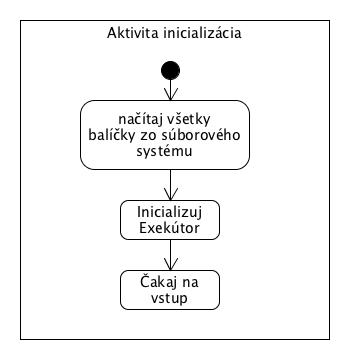
\includegraphics[scale=0.8]{img/initialization.jpg}
	\caption{Activita inicializácie aplikácie}
	\label{fig:test}
\end{figure}
\subsubsection{Načítanie pluginov}
\indent Načítanie pluginov sa uskutočňuje pomocou triedy PluginFactory a JarLoader, kde tento proces pozostáva z troch krokov.\newline
\paragraph{Načítanie dostupých pluginov z disku} Trieda PluginFactory zavolá metódu registerAllPlugins(), ktorá najprv získa cesty k uloženým jar súborom. Jar súbory musia byť uložené na presne špecifikovanom mieste. Následne tieto cesty odovzdá triede JarLoader, ktorá sa pokúsi na daných cestách načítať \acrshort{jar} súbory, nájsť v nich triedu implementujúcu rozhranie ShellPlugin. Ak takúto triedu nájde, pokúsi sa z nej vytvoriť inštanciu pomocou reflexie, a takto vytvorenú inštanciu následne vráti triede PluginFactory, ktorá si túto triedu uloží na základe informácií, ktoré každý ShellPlugin poskytuje. PluginFactory ukladá inštancie do mapy, kde kľúč je trieda PluginMeta získaná z pluginu, a hodnotou je práve načítaný plugin. 
\begin{algorithm}[H]
	\begin{minted}[]{java}
	try {
	URLClassLoader cl = URLClassLoader.newInstance(urls);
	JarInputStream jarFile = new JarInputStream(new FileInputStream(jarPath
	.toFile()));
	while (true) {
	jarEntry = jarFile.getNextJarEntry();
	if (jarEntry == null) {
	break;
	}
	if (jarEntry.getName().endsWith(".class")) {
	String className = jarEntry.getName()
	.substring(0, jarEntry.getName().length() - 6);
	className = className.replace('/', '.');
	Class c = cl.loadClass(className);
	Object obj = c.newInstance();
	if (obj instanceof ShellPlugin) {
	return Optional.of((ShellPlugin) obj);
	}
	}
	}
	\end{minted}
	\caption{Ukážka načítania balíčka z disku počítača}
	\label{alg:gen}
\end{algorithm}
\paragraph{Načítanie dostupých pluginov z aplikácie}
\indent Pluginy môžu byť definované priamo v aplikácii. V takom prípade, priamo do rovnakej mapy ako v predchádzajúcom prípade vkladáme inštancie pluginov a informácie o nich. 
\paragraph{Finálne načítanie pluginov}
\indent Používateľ môže počas využívania aplikácie stiahnuť alebo naprogramovať viaceré verzie rovnakého pluginu. Z tohto dôvodu sme navrhli  krok, ktorý má za úlohu načítať všetky balíčky s jedinečným menom a najvyššou možnou verziou pre daný balíček. Následne načítanie končí a vráti sa inštancia tejto továrne pre pluginy.
\subsection{Vykonávač príkazov}
\indent Všetky príkazy, ktoré sa majú pomocou aplikácie vykonať sa spúšťajú pomocou triedy ExecutorImpl, ktorá implementuje metódu rozhrania Executor CommandIO execute(String command, Scope scope). Rozhodovacia logika, ako sa príkazy od používateľa budú vykonávať, je implementovaná práve v tejto metóde. Pre zjednodušenie opisu si pomôžeme pseudokódom rozhodovacieho algoritmu. Zo pseudokódu je zrejmé, že exekútor najskôr zistí, či príkaz neobsahuje znaky pajpy, presmerovania štandardného vstupu/výstupu. Následne identifikuje čím sa príkaz začína a vyberie vhodnú metódu pre zadaný príkaz. Po vykonaní príkazu zisťuje či sa má výstup z programu zapísať mimo štandardného vstupu alebo výstupu. Ak áno, program očakáva platnú cestu za oddeľovačmi stdout> \acrshort{resp.} stderr>, kde sa pokúsi zapísať svoj výstup do súboru. Diagram tried je uvedený v prílohe D.
\begin{algorithm}[H]
	\begin{minted}[]{php}
	isPipe = isPipe(command);
	writeStd = shouldWriteStd(command);
	writeErr = shouldWriteErr(command);
	if (command.startsWith("sh ") 
	|| command.startsWith("win ") 
	|| command.startsWith("ext ")){
	  out = executeNativeCommand(command);
	}else if (command.startsWith("./"){
	  out = loadAndExecuteScript(command, scope);
	}else if (command.startsWith("${")) {
	  out = getVariable(command, scope);
	}else if (command.startsWith("$(")){
	if(isPipe){
	  executeCommandAsPipe(command, scope);
	}else{
	  executeCommand(command, scope);
	}
	}
	!writeStd ? saveToFile(out.getStdOut()) : out;
	!writeErr ? saveToFile(out.getErrOut()) : out;
	\end{minted}
	\caption{Ukážka pseudokódu exekútora. }
	\label{alg:gen}
\end{algorithm}
\newpage
\subsubsection{Vykonávač príkazu}
\indent Vykonávač príkazu si v prvom kroku vyžiada od PluginFactory plugin, ktorý by dokázal daný príkaz vykonať. Ak factory úspešne vráti plugin, exekútor si z pluginu zoberie command a zavolá na ňom metódu execute(CommandIO commandInput, Optional<Scope> scope). Command následne spracuje vstupy v metóde parseCommand(Stream<String> var). Metóda execute potom vyberie receiver, ktorý daný príkaz dokáže vykonať. Receiver následne vykoná príkaz a vráti rozhranie CommandIO, ktoré nesie informáciu o úspešnosti behu ako aj výstupy.

\subsubsection{Vykonávač pajpy}
\indent Ak aplikácia rozozná, že v príkaze ide o pajpu, príkaz putuje do triedy PipeExecutor, kde sa rozparsuje na parciálne príkazy. Po rozparsovaní príkazov sa každému príkazu nastaví nasledujúci príkaz, ktorý sa má vykonať. Posledný príkaz neobsahuje žiadny ďalší. Po takomto prednastavení exekútora sa spustí vykonávanie prvého príkazu, jeho výstup je pri úspešnom ukončení presmerovaný ďalšiemu príkazu. Tento kolobeh pokračuje až kým sa nedostane k poslednému príkazu. Ten následne vracia svoj výstup exekútorovi z 4.1.
\subsubsection{Vykonávač skriptu}
\indent Je popísaný v časti 4.1.2 tejto práce. Pre detailné pochopenie tejto metódy je potrebné prezrieť si priložené zdojové kódy aplikácie.
\subsection{Parser skriptov}
\indent Parser berie ako parameter cestu k skriptu, ktorý je potrebné sparsovať a vykonať. Parser skriptov pozostáva z dvoch častí: 
\begin{itemize}
	\item Predspracovania
	\item Parsovanie predspracovaného vstupu
\end{itemize}
\subsubsection{Predspracovanie}
\indent Úlohou predspracovania je načítať zdrojový kód skriptu, vyčistiť ho od komentárov, ako aj vyfiltrovať metódy, zistiť či skript obsahuje funkciu main, prípadne zmeniť používané pluginy. Predspracovanie pozostáva z viacerých krokov, ako prvé sa parser pokúsi načítať súbor po riadkoch ako stream zo Stringov. Ďalej zo súboru vyfiltruje všetky prázdne riadky, riadky obsahujúce komentáre, inak povedané začínajúce znakom mriežky. Z už vyfiltrovaných riadkov následne vyfiltrujeme iba tie, ktoré sa začínajú slovom use. Use slúži ako kľúčové slovo pre použitie pluginov v skriptoch. Pomocou týchto riadkov sa pokúsi vyžiadať od PluginFactory pluginy definované v use. Ak sa ich nepodarí nájsť aplikácia použije príkazy, ktoré má aktuálne k dispozícii, ale je pravdepodobné, že v tomto prípade dôjde ku chybe počas behu skriptu. Tieto riadky sa následne vymažú. Ďalší proces je filtrovanie riadkov, ktoré začínajú na kľúčové slovo include. Tieto riadky špecifikujú, ktoré ďalšie súbory sú použité v skripte. Rovnako ako pri use, riadky načítame do listu a zmažeme ich z hlavného obsahu. Ďalej načítame všetky súbory definované v include a pripojíme ich k tým, ktoré sme mali zo zdrojového skriptu. Načítavanie pomocou include sa deje cyklicky, avšak pamätáme si, ktoré súbory sme už načítali aby sme zabránili zacykleniu aplikácie a jej následnému pádu. Na záver si ešte vyfiltrujeme riadky začínajúce na function a zistíme unikátne mená definovaných funkcií. V prípade, že aplikácia nenájde funkciu main vyhodí výnimku a beh skriptu sa ukončí. Samozrejme používateľ je na túto skutočnosť upozornený. Po predspracovaní nasleduje parsovanie.
\subsubsection{Parsovanie}
\indent Aby sme si parsovanie skriptu vedeli jednoducho predstaviť, povedzme, že máme jeden for cyklus, ktorý prechádza cez všetky načítané riadky zo súborov. V tomto cykle následne definujeme rozhodovací mechanizmus, ktorý sa na základe prečítaného vstupu rozhodne čo má vykonať. Parser má za úlohu vytvárať scopy a pre vytvorené scopy získať podstatné informácie. Parser očakáva, že ak máme akékoľvek globálne príkazy v našom skripte, budú definované na začiatku skriptu. V momente ako parser narazí na prvú funkciu nenačítava príkazy do globálneho alebo skriptového scopu, ale do scopu konkrétnej funkcie. Parser tiež kontroluje či daná funkcia nemá pred sebou anotáciu @Override, v tomto prípade nastaví pre takúto funkciu príznak, že je prepísaná a mala by sa zobrať funkcia označená s @Override a nie pôvodná. Parser povoľuje aj viacnásobné prepísanie funkcie, do behu sa zoberie vždy tá, ktorá bola načítaná ako posledná. 
\subsubsection{Parsovanie funkcií}
\indent V momente, keď parser narazí na funkciu odovzdá riadenie ďalšej funkcii zodpovednej za správne načítanie funkcie. Parsovanie funkcie je zložitejší proces nakoľko môže dôjsť k rôznym situáciám. Na začiatku sa načíta prvý riadok, z neho sa vyparsuje návratová hodnota funkcie, meno funkcie a tiež parametre funkcie, kontroluje sa aj otváracia zátvorka pre scope, ktorá musí byť na riadku kde bola definovaná funkcia. Ďalšie riadky funkcie sa načítavajú v cykle a kontroluje sa nasledovné: 
\begin{itemize}	
	\item kontroluje sa správne ukončenie riadkov pomocou bodkočiarky.
	\item v prípade, že bol riadok ukončený bodkočiarkou, zisťuje sa či je na riadku definované volanie funkcie. Ak áno tento riadok je označený ako fcall s príslušným volaním funkcie a jej parametrami. V prípade, že nejde o volanie funkcie riadok sa označí ako volanie príkazu a to pomocou \$().
	\item v prípade, že je riadok ukončený s \\ parser pripojí k riadku nasledujúce riadky, pokým nenarazí na bodkočiarku.
	\item v prípade, že narazí na if odovzdá kontrolu parseru pre If scope, no predtým zapíše do aktuálneho scopu fcall s unikátnym identifikátorom podmienky.
	\item v prípade, že narazí na for odovzdá kontrolu parseru pre For scope, ale predtým zapíše do aktuálneho scopu fcall s unikátnym identifikátorom cyklu.
	\item v prípade, že narazí na return vytvorí príkaz, ktorý bude poskladaný z typ\_vracanej hodnoty returnType = hodnota za returnom;.
	\item  v prípade, že riadok obsahuje ukončovaciu kučeravú zátvorku, ukončí načítanie.
\end{itemize} 
\subsubsection{Parsovanie for cyklov}
\indent Ak hlavný parser odovzdá kontrolu parseru pre for cyklus, spustí sa preProcess funkcia v tomto scope, kde sa rozdielne načítava iba prvý riadok.
Z prvého riadku sa uložia tri parametre pre úspešný beh cyklu - počiatočná hodnota, podmienka, ktorá sa bude kontrolovať a inkrement. Pre vykonanie tejto úlohy je v scope vytvorená nová premenná, s unikátnym menom aby sa predišlo prepisovaniu premenných.
\subsubsection{Parsovanie podmienok}
\indent Ak hlavný parser odovzdá kontrolu parseru pre If podmienku, spustí sa preProcess funkcia v tomto scope, kde sa rozdielne načítava iba prvý riadok.
Z prvého riadku sa uloží iba jeden parameter a to podmienka, ktorá sa bude vždy vyhodnocovať.
\subsubsection{Výsledok parsovania}
\indent Výsledkom parsovania je štruktúra zobrazená na obrázku nižšie. V aplikačnom scope sa vytvorí scope skriptový, ktorý bude rodičom pre všetky ostatné scopy, ktoré sa vytvoria. Každý scope obsahuje stack príkazov, ktoré má vykonať počas behu. Tento stack môže obsahovať aj funkčné volania, ako je znázornené na obrázku. Po úspešnom ukončení parsovania sa na script scope zavolá funkcia main, ktorá spustí exekúciu skriptu.
\begin{figure}[!htbp]
	\centering
	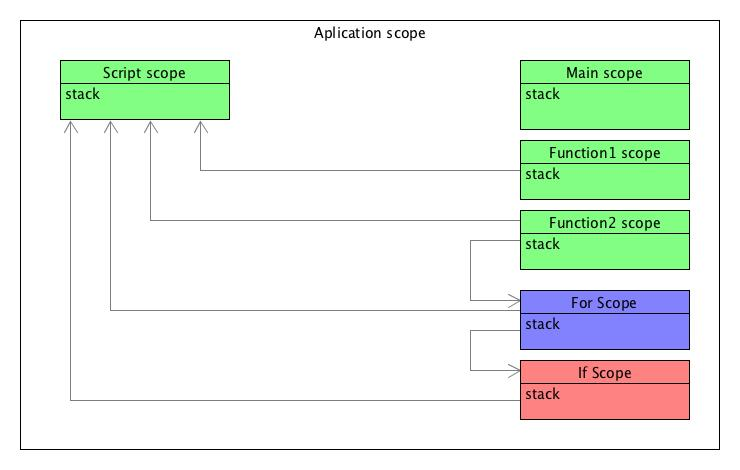
\includegraphics[width=\linewidth]{img/scopeStruct.jpg}
	\caption{Diagram tried rozhraní aplikácie}
	\label{fig:test}
\end{figure}
\subsection{Implementované pluginy}
\indent V tejto sekcii si stručne predstavíme naimplementované pluginy.
\section{Zhodnotenie výsledkov}
\indent Počas testovania aplikácie sme nenarazili na žiadne závažné problémy, pokiaľ sme dodržiavali zásady vymedzené v práci. 
\newline
\indent Aplikácia je schopná fungovať v troch rôznych režimoch, a to interaktívnom, skriptovacom a tiež v móde spúštania príkazov a skriptov priamo z konzoly pomocou parametrov. Taktiež je plne funkčná pri práci s premennými, skriptami, vykonávaním funkcií, cyklov a nami definovaných podmienok.
\newline
\indent  Podpora základných dátových typov je bezproblémová. Aritmetické operácie, ktoré je nad nimi možné vykonávať sú mierne okresané. Je možné definovať  operácie nad numerickými dátovými typmi ako +, -, *, /, \%, no nie je možné definovať ich prioritu. Rovnako to platí aj pre logické operátory ako \&\&, ||. Dobrou správou však je, že aj tieto funkcionality boli implementované pomocou pluginov a tým pádom je možné ich kedykoľvek nahradiť sofistikovanejšími riešeniami. 
\newline
\indent Tým, že je aplikácia postavená na Jave, je plne funkčná na každom \acrshort{pc}, ktorý má \acrshort{os} podporovaný touto platformou. Ako je možné vidieť z príručky, na spustenie aplikácie je potrebné iba nainštalovať Java JRE 8 , nastaviť Path aby smerovala na nainštalovanú Javu a spustiť predpripravený skript. Pre úplnosť sme pripravili nasledovné grafy, ktoré zobrazujú efektivitu aritmetických operácií.
